\documentclass[14pt]{extarticle}
\usepackage{fontspec}
\usepackage{polyglossia}
\usepackage{amsmath}
\usepackage{amssymb}
\usepackage{xcolor}
\usepackage{fancyhdr}
\usepackage{graphicx}
\usepackage{listings}
\usepackage[most]{tcolorbox}
% \usepackage{setspace}
\usepackage{pifont}
\usepackage{enumitem}
\usepackage{titlesec}
\usepackage[bottom]{footmisc}
\usepackage{titling}
\usepackage{minted}
\usepackage{etoolbox}
\usepackage{array}
\usepackage{extsizes}
\usepackage{float}
\usepackage{booktabs}
\usepackage{hyperref}
\usepackage[onehalfspacing]{setspace}
\usepackage[a4paper, top=2.7cm, bottom=2.7cm, left=2.5cm, right=2.5cm, headheight=1.5cm, headsep=0.5cm]{geometry}
\usepackage{tikz}

\usetikzlibrary{automata, positioning, arrows.meta, arrows}

\newfontfamily\emoji{Segoe UI Emoji}

\pagestyle{fancy}

\setmainlanguage[numerals=western]{arabic}
\setotherlanguage{english}
% \newfontfamily\arabicfont[Script=Arabic]{Amiri}
\newfontfamily\arabicfont[Script=Arabic]{Calibri}
\newfontfamily\arabicfonttt[Script=Arabic]{Courier New}

\lstset{
  language=[Sharp]C,
  numbers=left,
  stepnumber=1,
  numbersep=8pt,
  frame=single,
  basicstyle=\ttfamily\small,
  keywordstyle=\color{blue},
  stringstyle=\color{red},
  commentstyle=\color{green!50!black}
}

\newif\ifdetailed
\ifdefined\setdetailed
  \setdetailed
\fi

\newif\ifwithsols
\ifdefined\setwithsols
  \setwithsols
\fi

% unified tcolorboxes for articles
\tcbset{colback=white, colframe=black, fonttitle=\bfseries, boxrule=0.8pt}
\newtcolorbox{boxDef}[1][]{colback=blue!5!white,colframe=blue!75!black,
  title={{\emoji📘} تعريف\ifx\\#1\\\else ~#1\fi :}}
\newtcolorbox{boxExercise}[1][]{colback=cyan!5!white,colframe=cyan!70!black,
  title={{\emoji🧩} تمرين\ifx\\#1\\\else ~#1\fi :}}
\newtcolorbox{boxExample}[1][]{colback=yellow!5!white,colframe=orange!90!black,
  title={{\emoji📝} مثال\ifx\\#1\\\else ~#1\fi :}}
\newtcolorbox{boxNote}[1][]{colback=gray!10!white,colframe=black,
  title={{\emoji✨} ملاحظة\ifx\\#1\\\else ~#1\fi :}}
\newtcolorbox{boxAttention}[1][]{colback=magenta!10!white,colframe=magenta!80!black,
  title={{\emoji🔔} تنبيه\ifx\\#1\\\else ~#1\fi :}}
\newtcolorbox{boxWarning}[1][]{colback=red!5!white,colframe=red!75!black,
  title={{\emoji⚡} ملاحظة هامة\ifx\\#1\\\else ~#1\fi :}}
\newtcolorbox{boxSolution}[1][]{colback=green!5!white,colframe=green!60!black,
  title={{\emoji✅} حل\ifx\\#1\\\else ~#1\fi :}}
\newtcolorbox{boxSymbol}[1][]{colback=purple!5!white,colframe=purple!70!black,
  title={{\emoji🔣} رمز\ifx\\#1\\\else ~#1\fi :}}
\newtcolorbox{boxHint}[1][]{colback=teal!5!white,colframe=teal!60!black,
  title={{\emoji💡} تلميح\ifx\\#1\\\else ~#1\fi :}}


\tcbset{simplecode/.style={ colback=gray!5, colframe=black!50, boxrule=0.4pt, arc=2pt, left=4pt,right=4pt,top=4pt,bottom=4pt}}
\newenvironment{boxCode}{\begin{tcolorbox}[simplecode]}{\end{tcolorbox}}

\newcolumntype{C}[1]{>{\centering\arraybackslash}p{#1}}

% redefine spaces after titles
\makeatletter
\renewcommand{\@maketitle}{%
  \begin{center}
    {\huge \bfseries \@title \par}%
    \vskip 0.2em % space between title and author
    {\large \@author \par}%
    % \vskip 0.2em % space between author and date
    % {\normalsize \@date \par}%
  \end{center}
}
\makeatother

\fancyhf{} % clear default
\fancypagestyle{plain}{
  \fancyhf{}
  \fancyhead[L]{مدرسة التسامح الشاملة}
  % \fancyhead[L]{
\includegraphics[height=1cm]{../../../images/logoTasamoh.png}}
  \fancyhead[R]{الأستاذ محمود اغبارية}
  \fancyfoot[C]{\thepage}
}

\fancyhead[L]{مدرسة التسامح الشاملة}
\fancyhead[R]{الأستاذ محمود اغبارية}
\fancyfoot[C]{\thepage}
% \date{\today}

\setcounter{tocdepth}{3} % only section subsection and subsubsection in TOC

\newcommand{\importpdfpage}[2]{%
    \thispagestyle{empty}
    \newgeometry{left=0cm,right=0cm,top=0cm,bottom=0cm}
    \includegraphics[page=#2,width=0.95\paperwidth,height=0.95\paperheight,keepaspectratio]{#1}
    \restoregeometry
}

\newcommand{\insertFullImg}[1]{%
    \noindent
    \makebox[\textwidth][c]{
        \includegraphics[width=0.9\paperwidth,keepaspectratio]{#1}%
    }%
}%

% ----------------------


% \begin{document}

% \maketitle

% % \clearpage  % start TOC on a new page
% % \renewcommand{\contentsname}{جدول المحتويات}
% % \tableofcontents
% % \clearpage

% \part*{part 1} % the * prevents numbering
% \section*{مقدمة}
% \subsection*{مثال رياضي}
% \subsubsection*{مثال فرعي}
% \paragraph*{ paragraph 1}
% \subparagraph*{sub paragraph 1}

% \ifdetailed
% \begin{english}
% \begin{minted}{csharp}
% // C# Example
% \end{minted}
% \end{english}
% \fi

% OLD WAY
% \ifdetailed
% \begin{english}
% \begin{lstlisting}
% // C# Example
% \end{lstlisting}
% \end{english}
% \fi

% % 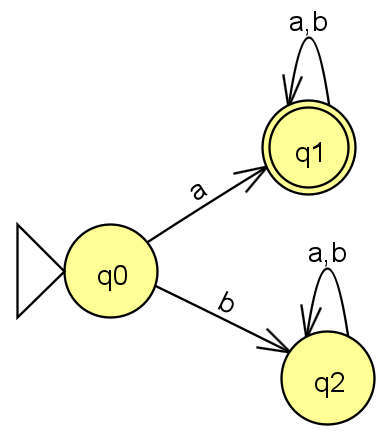
\includegraphics[width=0.2\textwidth]{../../../images/DFAs/ex1_q1.png}



% \vspace{3cm}
% \begin{flushleft}
% أرجو لكم وقتًا ممتعًا.

% الأستاذ محمود اغبارية.
% \end{flushleft}


% \end{document}


\ifwithsols
\title{حل اختبار فصلي \\ الصف العاشر 10}
\else
\title{اختبار فصلي \\ الصف العاشر 10}
\fi

\begin{document}

\maketitle
\thispagestyle{fancy}

%% 1. متابعة أساسي - 10 علامات
%% 2. متابعة مصفوفة كائنات + كتابة كود اساسي لتعريفها - 25 علامة
%% 3. سؤال مصفوفات جيد - 20 علامة
%% 4. سؤال مصفوفة كائنات - 25 علامة
%% 5. سؤال فئات جامد - 30 علامة

\section{الفصل الأول}
\input{../../../bagrut_questions/basics/arrays_2025_899371_1.tex}
\input{../../../bagrut_questions/basics/classes0_2020_899381b_1.tex}
% \input{../../../bagrut_questions/basics/loops_for_2008_899222_10.tex}
% \subsection*{سؤال 7 امتحان 899222 سنة 2010}
\addcontentsline{toc}{subsection}{سؤال 7 امتحان 899222 سنة 2010}

\noindent
\makebox[\textwidth][c]{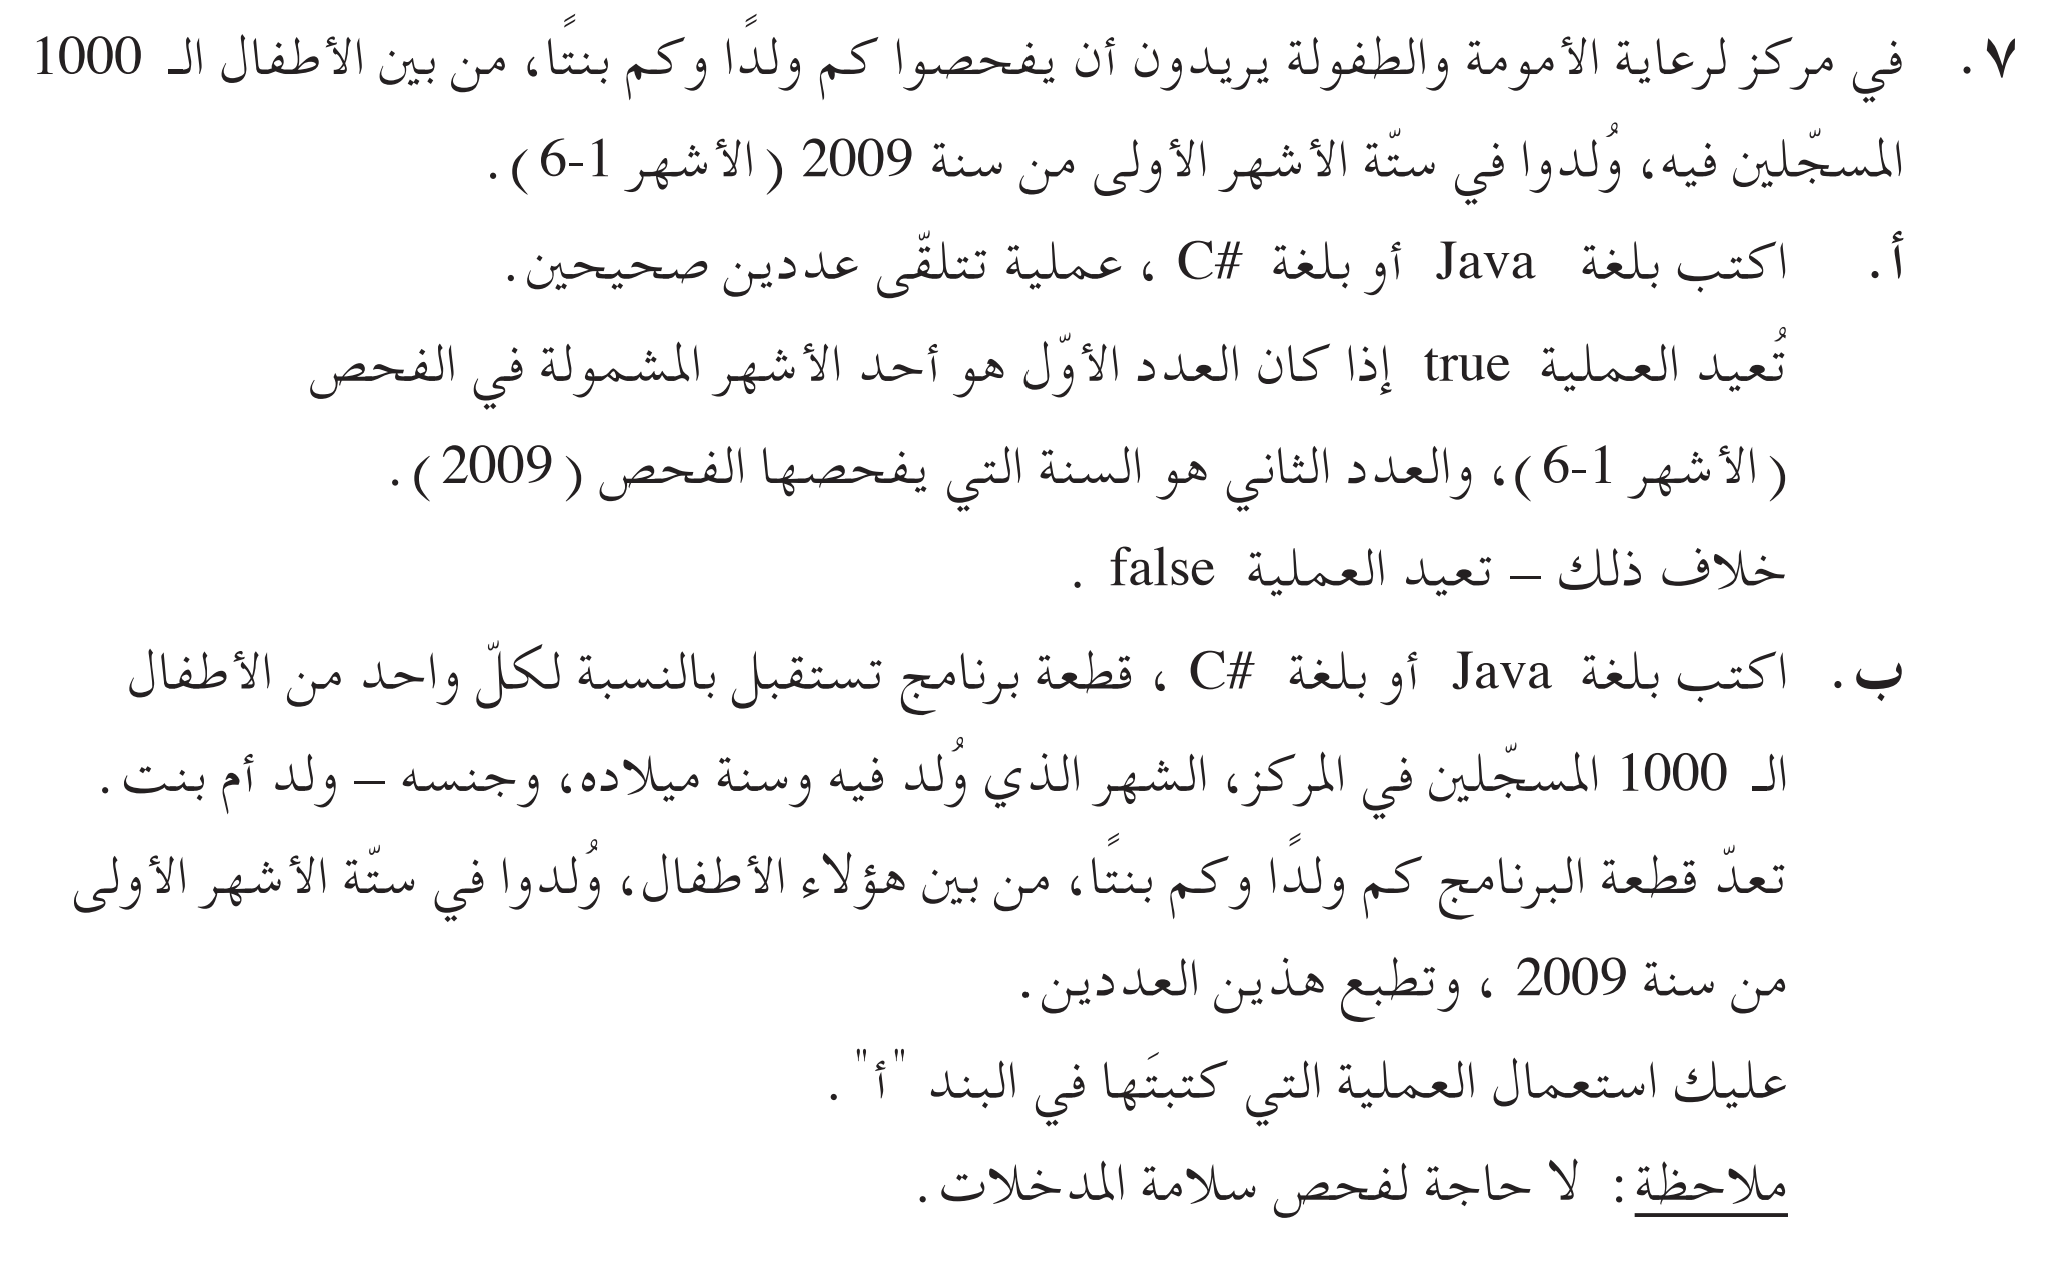
\includegraphics[width=0.9\paperwidth,keepaspectratio]{ ../../../bagrut_questions/basics/loops_for_2010_899222_7.png }%
}%


% \ifwithsols
% \begin{boxSolution}[سؤال 7 امتحان 899222 سنة 2010]
% \begin{enumerate}[itemsep=1.5em, label=\alph*.]
%     \item // TODO:

% \end{enumerate}

% \begin{boxCode}
% \begin{english}
% \begin{minted}{csharp}
%     // TODO
% \end{minted}
% \end{english}
% \end{boxCode}

% \end{boxSolution}
% \clearpage
% \fi


\section{الفصل الثاني}
% \subsection*{سؤال 2 امتحان 899222 سنة 2017}
\addcontentsline{toc}{subsection}{سؤال 2 امتحان 899222 سنة 2017}

\noindent
\makebox[\textwidth][c]{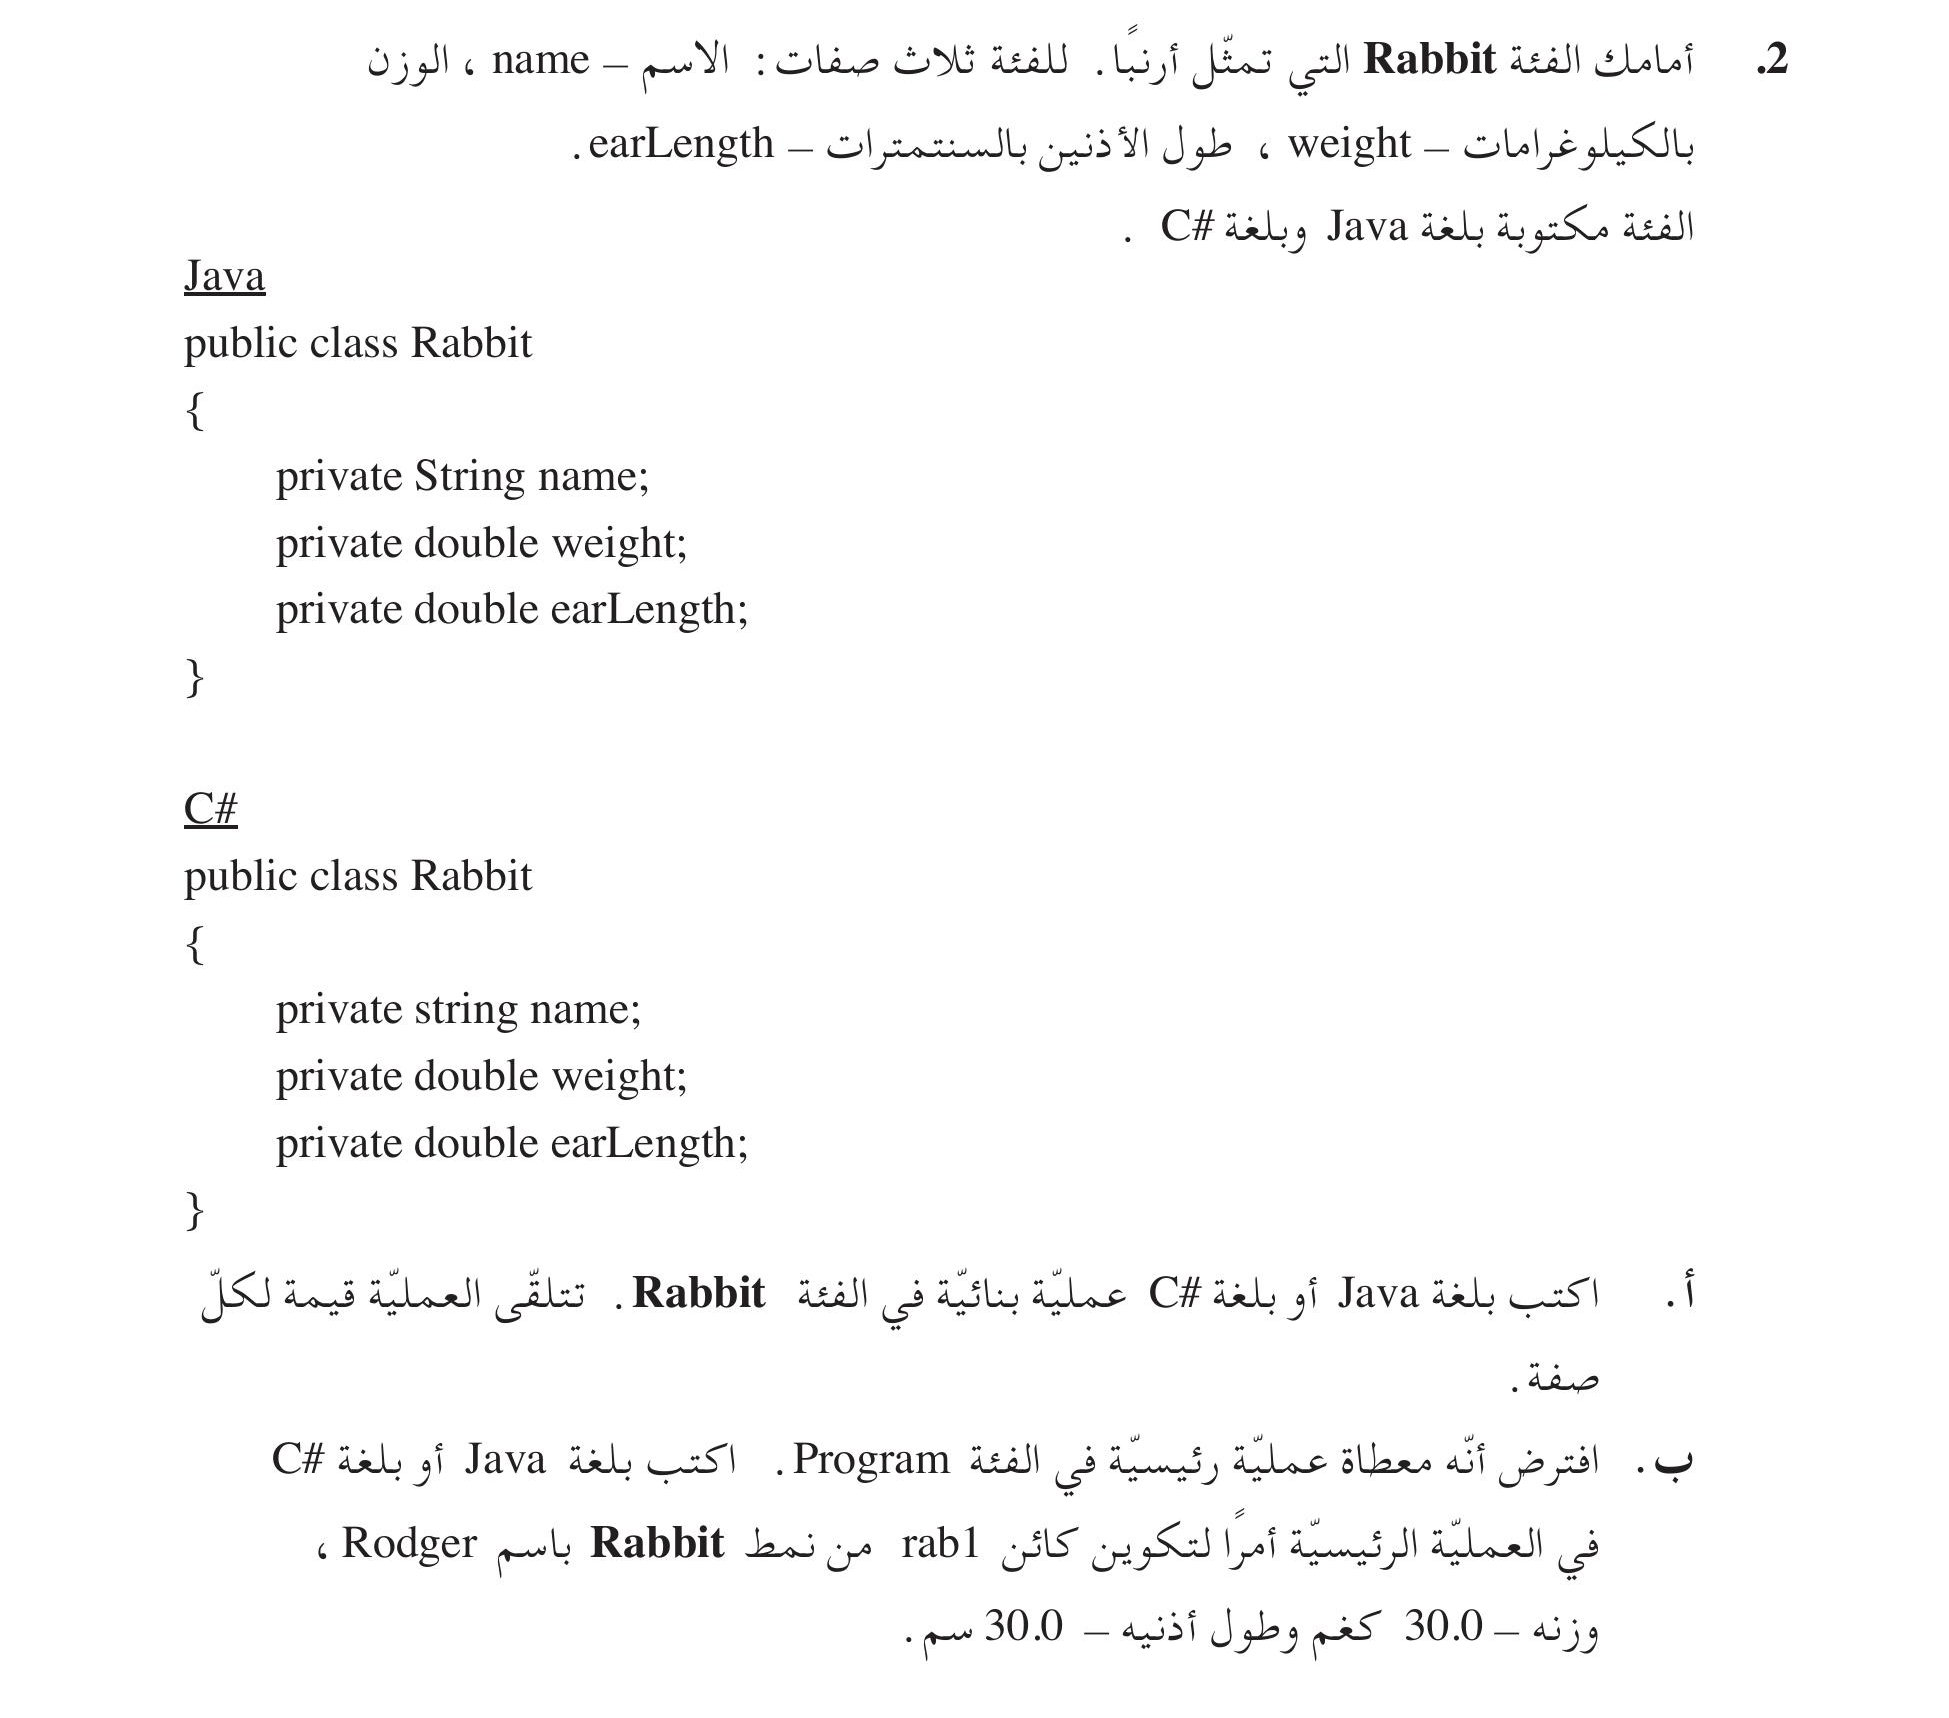
\includegraphics[width=0.9\paperwidth,keepaspectratio]{ ../../../bagrut_questions/basics/classes0_2017_899222_2.jpg }%
}%


% \ifwithsols
% \begin{boxSolution}[سؤال 2 امتحان 899222 سنة 2017]
% \begin{enumerate}[itemsep=1.5em, label=\alph*.]
%     \item // TODO:

% \end{enumerate}

% \begin{boxCode}
% \begin{english}
% \begin{minted}{csharp}
%     // TODO
% \end{minted}
% \end{english}
% \end{boxCode}

% \end{boxSolution}
% \clearpage
% \fi

\subsection*{سؤال 10 امتحان 899222 سنة 2014}
\addcontentsline{toc}{subsection}{سؤال 10 امتحان 899222 سنة 2014}

\noindent
\makebox[\textwidth][c]{
\includegraphics[width=0.9\paperwidth,keepaspectratio]{ ../../../bagrut_questions/basics/arrays_2014_899222_10.jpg }%
}%


\ifwithsols
{\small
\begin{boxSolution}[سؤال 10 امتحان 899222 سنة 2014]
\begin{boxCode}
\begin{english}
\begin{minted}{csharp}
class Program
{
    public static int Discount(int members, int students)
    {
        int d1 = 0;
        int d2 = students * 40;
        if (members > 6)
            d1 = 100;
        if (d1 > d2)
            return d1;
        return d2;
    }

    public static int TownDiscount(int numFamilies)
    {
        int total = 0;
        for (int i = 0; i < numFamilies; i++)
        {
            int members = int.Parse(Console.ReadLine());
            int students = int.Parse(Console.ReadLine());
            total += Discount(members, students);
        }
        return total;
    }

    public static void Main(string[] args)
    {
        int[] rdc = new int[10];
        for (int i = 0; i < 10; i++)
        {
            int numFamilies = int.Parse(Console.ReadLine());
            int total = TownDiscount(numFamilies);
            if (total > rdc[i])
                Console.WriteLine(i);
        }
    }
}
\end{minted}
\end{english}
\end{boxCode}
\end{boxSolution}
}
\clearpage
\fi

\subsection*{سؤال 8 امتحان 899222 سنة 2017}
\addcontentsline{toc}{subsection}{سؤال 8 امتحان 899222 سنة 2017}

\noindent
\makebox[\textwidth][c]{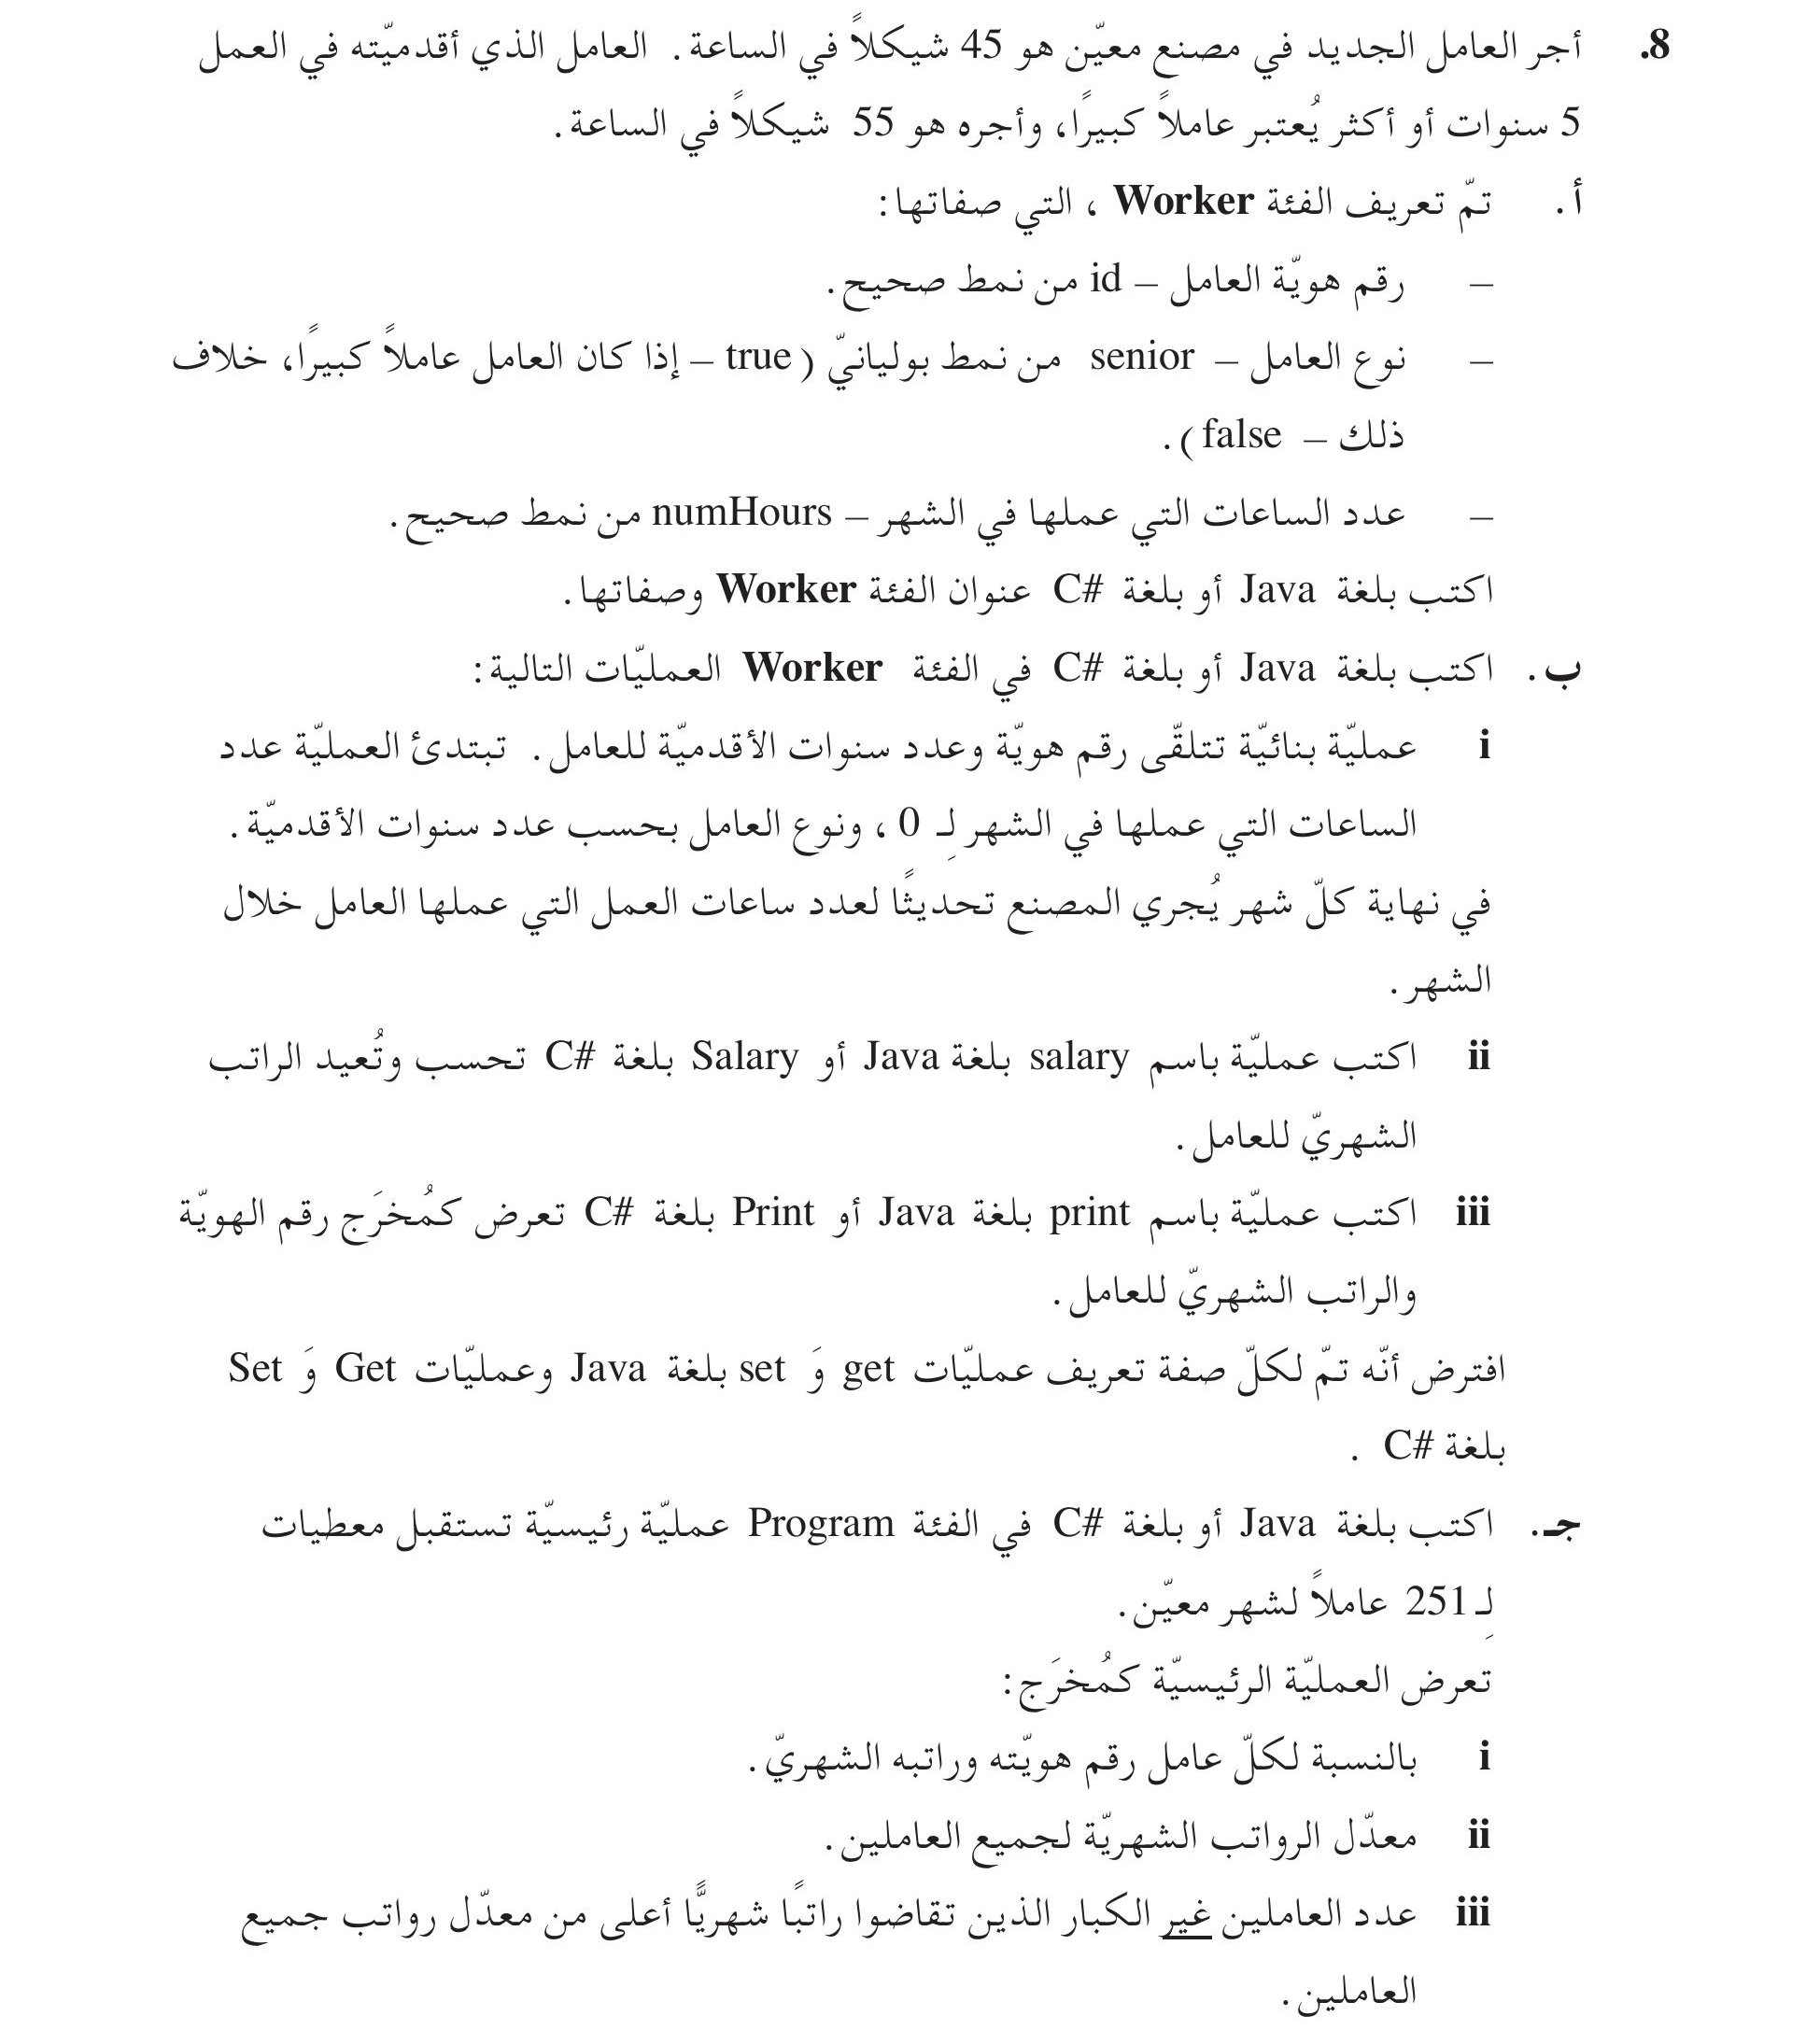
\includegraphics[width=0.9\paperwidth,keepaspectratio]{ ../../../bagrut_questions/basics/classes1_2017_899222_8.jpg }%
}%


\ifwithsols
{\small
\begin{boxSolution}[سؤال 8 امتحان 899222 سنة 2017]
\begin{boxCode}
\begin{english}
\begin{minted}{csharp}
class Worker
{
    private int id;
    private bool senior;
    private int numHours;

    public Worker(int id, int years)
    {
        this.id = id;
        if (years >= 5)
            this.senior = true;
        else
            this.senior = false;
        this.numHours = 0;
    }

    public int Salary()
    {
        if (this.senior)
            return this.numHours * 55;
        return this.numHours * 45;
    }

    public void Print()
    {
        Console.WriteLine(this.id + " " + this.Salary());
    }
    public void SetNumHours(int numHours) { this.numHours = numHours; }
    public bool GetSenior() { return this.senior; }
}
\end{minted}
\end{english}
\end{boxCode}
\end{boxSolution}

\begin{boxSolution}[سؤال 8 امتحان 899222 سنة 2017 - تكملة]
\begin{boxCode}
\begin{english}
\begin{minted}{csharp}
class Program
{
    public static void Main(string[] args)
    {
        Worker[] arr = new Worker[251];
        int sum = 0;

        for (int i = 0; i < 251; i++)
        {
            int id = int.Parse(Console.ReadLine());
            int years = int.Parse(Console.ReadLine());
            int hours = int.Parse(Console.ReadLine());

            arr[i] = new Worker(id, years);
            arr[i].SetNumHours(hours);

            arr[i].Print();
            sum += arr[i].Salary();
        }

        double avg = (double)sum / 251;
        Console.WriteLine(avg);

        int count = 0;
        for (int i = 0; i < 251; i++)
        {
            if (!arr[i].GetSenior() && arr[i].Salary() > avg)
            {
                count++;
            }
        }
        Console.WriteLine(count);
    }
}
\end{minted}
\end{english}
\end{boxCode}
\end{boxSolution}
}
\clearpage
\fi

\subsection*{سؤال 9 امتحان 899222 سنة 2017}
\addcontentsline{toc}{subsection}{سؤال 9 امتحان 899222 سنة 2017}

\noindent
\makebox[\textwidth][c]{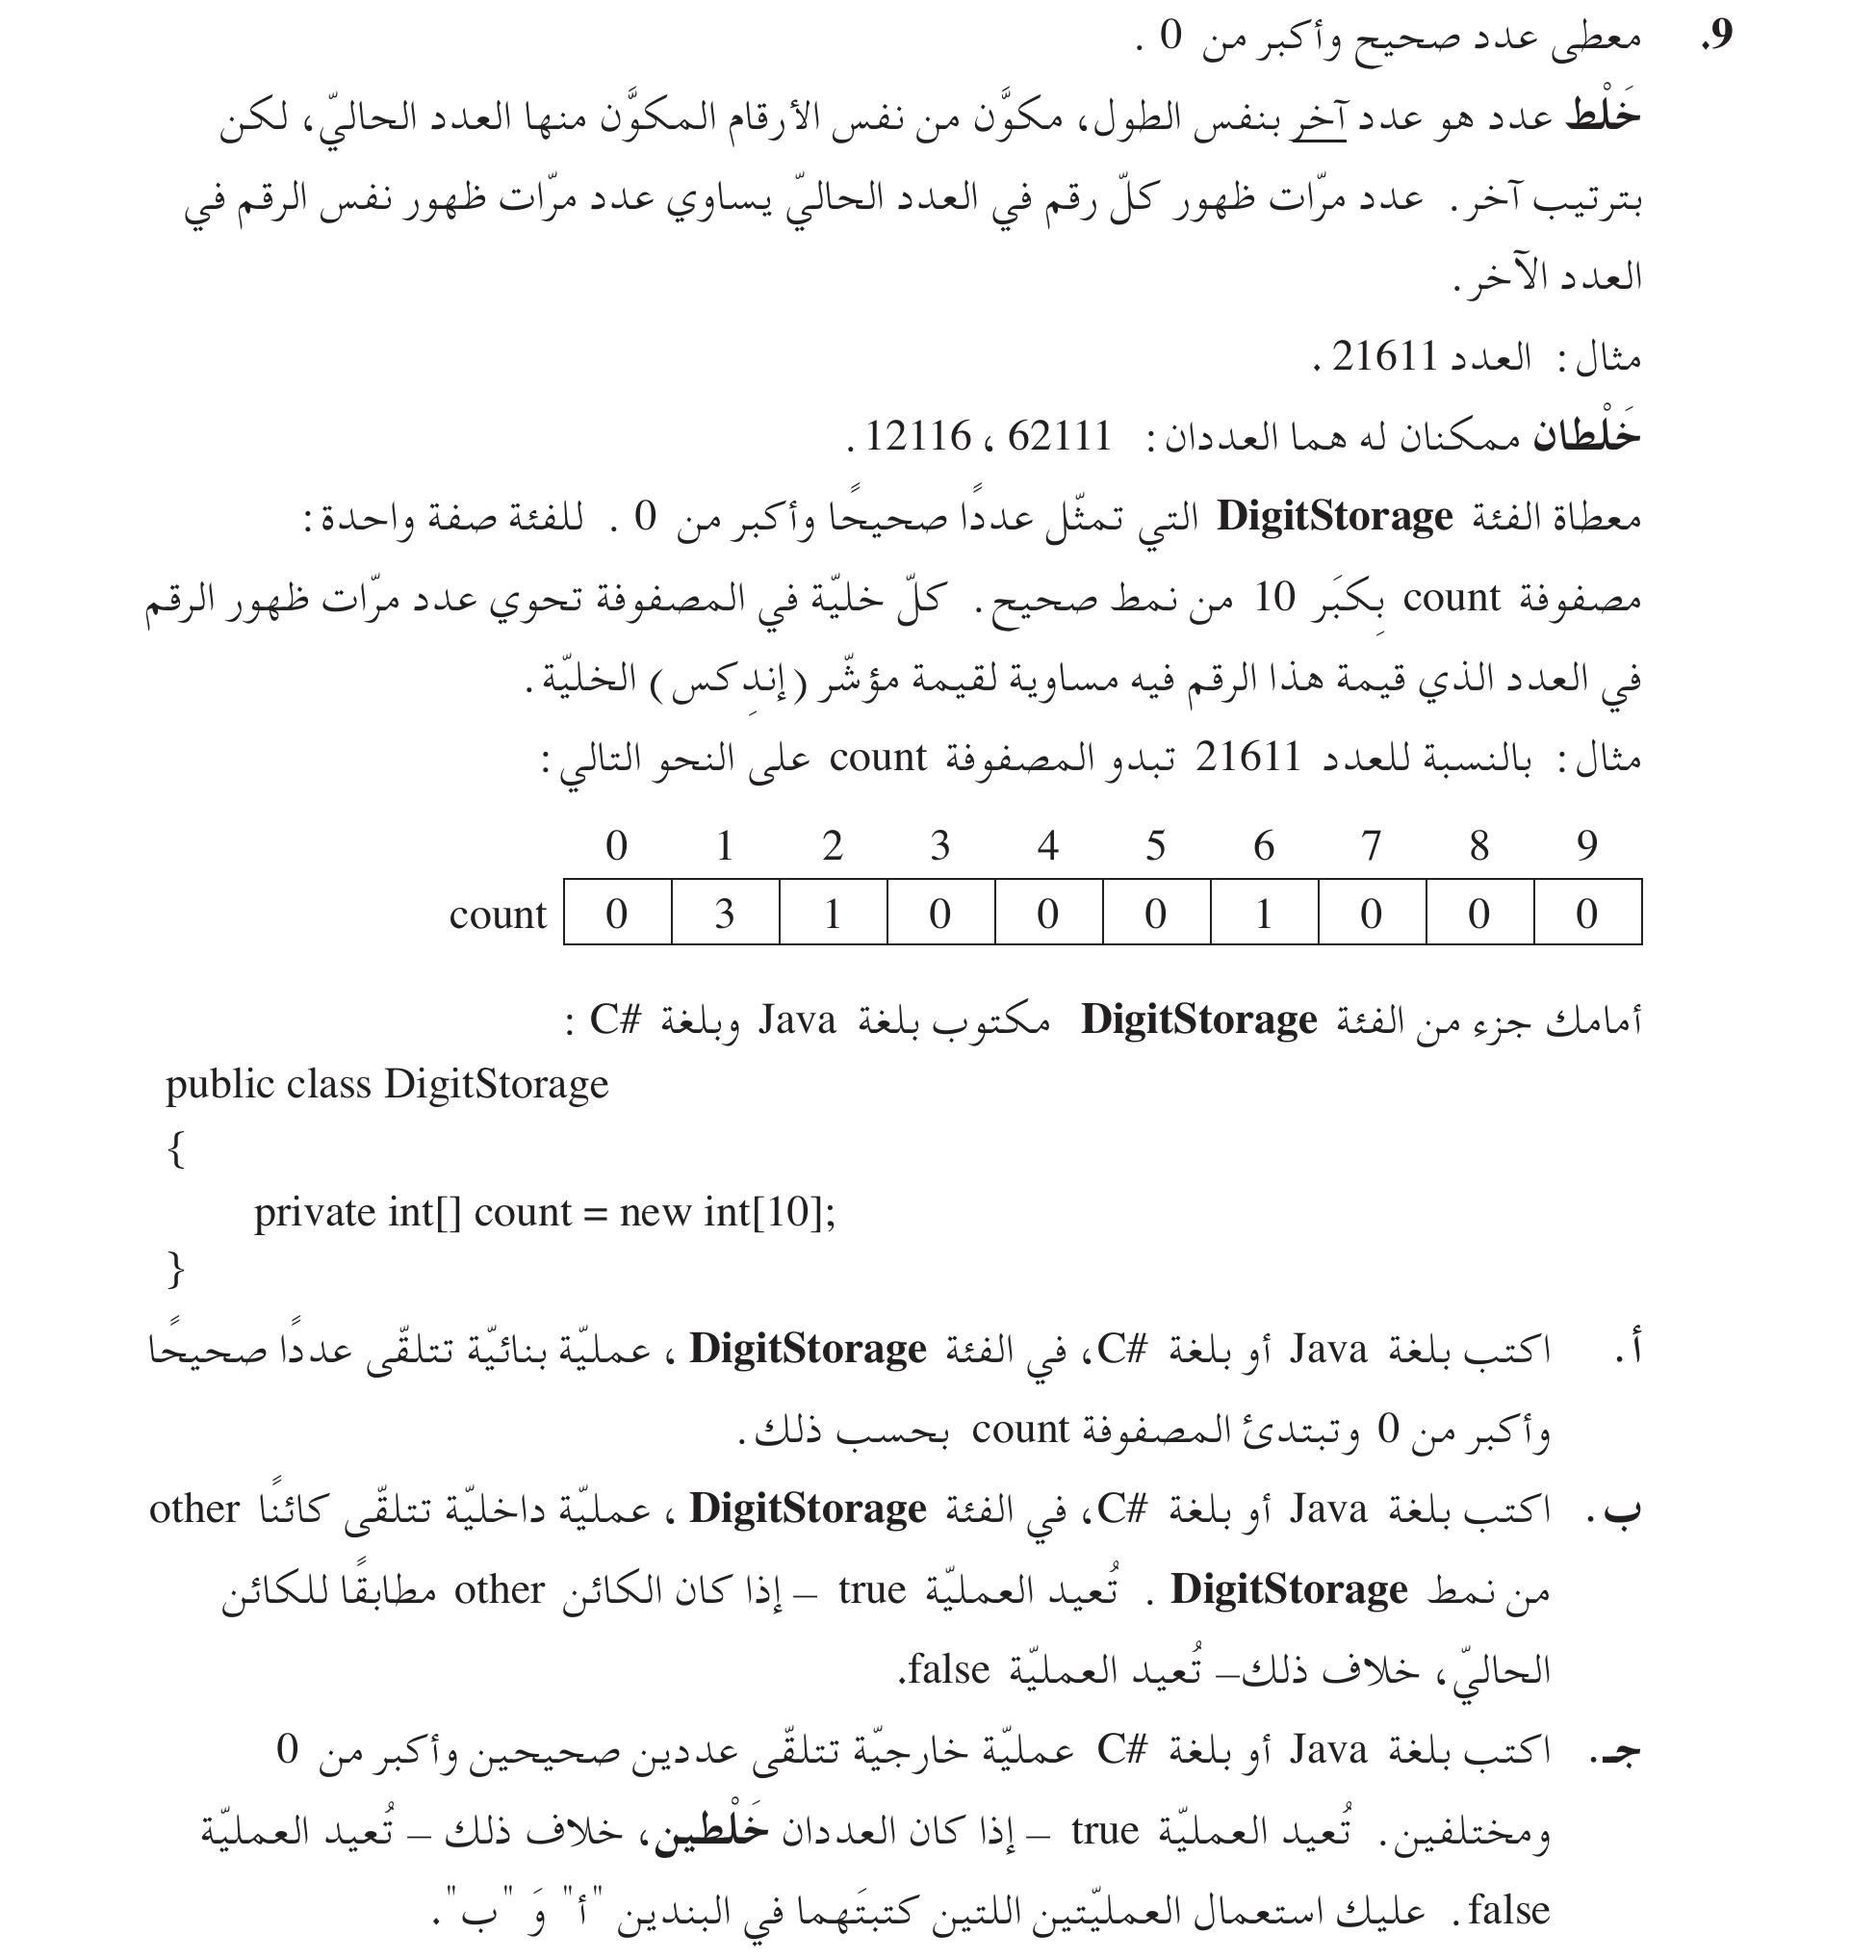
\includegraphics[width=0.9\paperwidth,keepaspectratio]{ ../../../bagrut_questions/basics/classes2_2017_899222_9.jpg }%
}%


\ifwithsols
{\small
\begin{boxSolution}[سؤال 9 امتحان 899222 سنة 2017]
\begin{boxCode}
\begin{english}
\begin{minted}{csharp}
public class DigitStorage
{
    private int[] count = new int[10];

    public DigitStorage(int num)
    {
        while (num > 0)
        {
            this.count[num % 10]++;
            num = num / 10;
        }
    }

    public bool IsIdentical(DigitStorage other)
    {
        for (int i = 0; i < 10; i++)
        {
            if (this.count[i] != other.count[i])
                return false;
        }
        return true;
    }
}

class Program
{
    public static bool IsMix(int num1, int num2)
    {
        DigitStorage d1 = new DigitStorage(num1);
        DigitStorage d2 = new DigitStorage(num2);

        return d1.IsIdentical(d2);
    }
}
\end{minted}
\end{english}
\end{boxCode}
\end{boxSolution}
}
\clearpage
\fi

% \input{../../../bagrut_questions/basics/classes2_2020_899381b_2.tex}

\end{document}



% \documentclass[14pt]{extarticle}
% \usepackage{fontspec}
\usepackage{polyglossia}
\usepackage{amsmath}
\usepackage{amssymb}
\usepackage{xcolor}
\usepackage{fancyhdr}
\usepackage{graphicx}
\usepackage{listings}
\usepackage[most]{tcolorbox}
% \usepackage{setspace}
\usepackage{pifont}
\usepackage{enumitem}
\usepackage{titlesec}
\usepackage[bottom]{footmisc}
\usepackage{titling}
\usepackage{minted}
\usepackage{etoolbox}
\usepackage{array}
\usepackage{extsizes}
\usepackage{float}
\usepackage{booktabs}
\usepackage{hyperref}
\usepackage[onehalfspacing]{setspace}
\usepackage[a4paper, top=2.7cm, bottom=2.7cm, left=2.5cm, right=2.5cm, headheight=1.5cm, headsep=0.5cm]{geometry}
\usepackage{tikz}

\usetikzlibrary{automata, positioning, arrows.meta, arrows}

\newfontfamily\emoji{Segoe UI Emoji}

\pagestyle{fancy}

\setmainlanguage[numerals=western]{arabic}
\setotherlanguage{english}
% \newfontfamily\arabicfont[Script=Arabic]{Amiri}
\newfontfamily\arabicfont[Script=Arabic]{Calibri}
\newfontfamily\arabicfonttt[Script=Arabic]{Courier New}

\lstset{
  language=[Sharp]C,
  numbers=left,
  stepnumber=1,
  numbersep=8pt,
  frame=single,
  basicstyle=\ttfamily\small,
  keywordstyle=\color{blue},
  stringstyle=\color{red},
  commentstyle=\color{green!50!black}
}

\newif\ifdetailed
\ifdefined\setdetailed
  \setdetailed
\fi

\newif\ifwithsols
\ifdefined\setwithsols
  \setwithsols
\fi

% unified tcolorboxes for articles
\tcbset{colback=white, colframe=black, fonttitle=\bfseries, boxrule=0.8pt}
\newtcolorbox{boxDef}[1][]{colback=blue!5!white,colframe=blue!75!black,
  title={{\emoji📘} تعريف\ifx\\#1\\\else ~#1\fi :}}
\newtcolorbox{boxExercise}[1][]{colback=cyan!5!white,colframe=cyan!70!black,
  title={{\emoji🧩} تمرين\ifx\\#1\\\else ~#1\fi :}}
\newtcolorbox{boxExample}[1][]{colback=yellow!5!white,colframe=orange!90!black,
  title={{\emoji📝} مثال\ifx\\#1\\\else ~#1\fi :}}
\newtcolorbox{boxNote}[1][]{colback=gray!10!white,colframe=black,
  title={{\emoji✨} ملاحظة\ifx\\#1\\\else ~#1\fi :}}
\newtcolorbox{boxAttention}[1][]{colback=magenta!10!white,colframe=magenta!80!black,
  title={{\emoji🔔} تنبيه\ifx\\#1\\\else ~#1\fi :}}
\newtcolorbox{boxWarning}[1][]{colback=red!5!white,colframe=red!75!black,
  title={{\emoji⚡} ملاحظة هامة\ifx\\#1\\\else ~#1\fi :}}
\newtcolorbox{boxSolution}[1][]{colback=green!5!white,colframe=green!60!black,
  title={{\emoji✅} حل\ifx\\#1\\\else ~#1\fi :}}
\newtcolorbox{boxSymbol}[1][]{colback=purple!5!white,colframe=purple!70!black,
  title={{\emoji🔣} رمز\ifx\\#1\\\else ~#1\fi :}}
\newtcolorbox{boxHint}[1][]{colback=teal!5!white,colframe=teal!60!black,
  title={{\emoji💡} تلميح\ifx\\#1\\\else ~#1\fi :}}


\tcbset{simplecode/.style={ colback=gray!5, colframe=black!50, boxrule=0.4pt, arc=2pt, left=4pt,right=4pt,top=4pt,bottom=4pt}}
\newenvironment{boxCode}{\begin{tcolorbox}[simplecode]}{\end{tcolorbox}}

\newcolumntype{C}[1]{>{\centering\arraybackslash}p{#1}}

% redefine spaces after titles
\makeatletter
\renewcommand{\@maketitle}{%
  \begin{center}
    {\huge \bfseries \@title \par}%
    \vskip 0.2em % space between title and author
    {\large \@author \par}%
    % \vskip 0.2em % space between author and date
    % {\normalsize \@date \par}%
  \end{center}
}
\makeatother

\fancyhf{} % clear default
\fancypagestyle{plain}{
  \fancyhf{}
  \fancyhead[L]{مدرسة التسامح الشاملة}
  % \fancyhead[L]{
\includegraphics[height=1cm]{../../../images/logoTasamoh.png}}
  \fancyhead[R]{الأستاذ محمود اغبارية}
  \fancyfoot[C]{\thepage}
}

\fancyhead[L]{مدرسة التسامح الشاملة}
\fancyhead[R]{الأستاذ محمود اغبارية}
\fancyfoot[C]{\thepage}
% \date{\today}

\setcounter{tocdepth}{3} % only section subsection and subsubsection in TOC

\newcommand{\importpdfpage}[2]{%
    \thispagestyle{empty}
    \newgeometry{left=0cm,right=0cm,top=0cm,bottom=0cm}
    \includegraphics[page=#2,width=0.95\paperwidth,height=0.95\paperheight,keepaspectratio]{#1}
    \restoregeometry
}

\newcommand{\insertFullImg}[1]{%
    \noindent
    \makebox[\textwidth][c]{
        \includegraphics[width=0.9\paperwidth,keepaspectratio]{#1}%
    }%
}%

% ----------------------


% \begin{document}

% \maketitle

% % \clearpage  % start TOC on a new page
% % \renewcommand{\contentsname}{جدول المحتويات}
% % \tableofcontents
% % \clearpage

% \part*{part 1} % the * prevents numbering
% \section*{مقدمة}
% \subsection*{مثال رياضي}
% \subsubsection*{مثال فرعي}
% \paragraph*{ paragraph 1}
% \subparagraph*{sub paragraph 1}

% \ifdetailed
% \begin{english}
% \begin{minted}{csharp}
% // C# Example
% \end{minted}
% \end{english}
% \fi

% OLD WAY
% \ifdetailed
% \begin{english}
% \begin{lstlisting}
% // C# Example
% \end{lstlisting}
% \end{english}
% \fi

% % 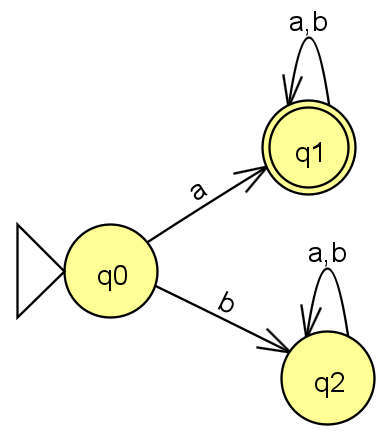
\includegraphics[width=0.2\textwidth]{../../../images/DFAs/ex1_q1.png}



% \vspace{3cm}
% \begin{flushleft}
% أرجو لكم وقتًا ممتعًا.

% الأستاذ محمود اغبارية.
% \end{flushleft}


% \end{document}


% \ifwithsols
% \title{حل اختبار فصلي \\ الصف العاشر 10}
% \else
% \title{اختبار فصلي \\ الصف العاشر 10}
% \fi

% \begin{document}

% \maketitle

% \begin{flushleft}
%     $02.06.2026$
% \end{flushleft}

% \ifwithsols
% \else
% \begin{boxCode}
%     \begin{itemize}
%         \item \textbf{الاختبار مكوّن من فصلين:}
%         \begin{itemize}
%             \item \textbf{الفصل الأول:} يحتوي على سؤالين 1 و2 - أجب عن كلا السؤالين.
%             \item \textbf{الفصل الثاني:} يحتوي على ثلاثة أسئلة 3-5 - أجب عن سؤالين فقط.
%         \end{itemize}
%         \item الوقت المخصص: ساعتان.
%         \item يسمح باستخدام كل مادة مساعدة، عدا الآلة التي يمكن برمجتها.
%         \item اكتب بقلم حبر فقط، وبخط واضح.
%         \item الحل على ورقة خارجية، لا تنسَ كتابة اسمك.
%         \item مرفق ورقة خاصة لتسليم حل السؤالين الأول والثاني (جدول المتابعة)
%     \end{itemize}
% \end{boxCode}

% \begin{center}
%   
\includegraphics[width=0.4\textwidth]{../../../images/logoTasamoh.png}
% \end{center}

% \vspace{2cm}
% \begin{flushleft}
%     أرجو لكم التفوّق.

%     الأستاذ محمود اغبارية.
% \end{flushleft}
% \clearpage
% \fi

% %%%%%%%%%%%%%%%%%%%%%%%%%%%%%%%%%%%%
% \section*{الفصل الأول}

% \textbf{السؤال الأول} (15 علامة) \\
% أمامك العملية \textenglish{What} التالية:

% \begin{boxCode}
% \begin{english}
% \begin{minted}{csharp}
% public static int What(int[] arr)
% {
%     int y = 0;
%     int x = arr[0];
%     for (int i = 0; i < arr.Length; i++)
%     {
%         y += arr[i];
%         x = Math.Max(x, y);
%         y = Math.Max(y, 0);
%     }
%     return x;
% }
% \end{minted}
% \end{english}
% \end{boxCode}

% معطاة المصفوفة \textenglish{arr}:

% {\small
% \begin{english}
% \begin{center}
% \renewcommand{\arraystretch}{1.5}
% \setlength{\tabcolsep}{12pt}
% \begin{tabular}{c | c | c | c | c | c | c |}
% \multicolumn{1}{c}{} & \multicolumn{1}{c}{0} & \multicolumn{1}{c}{1} & \multicolumn{1}{c}{2} & \multicolumn{1}{c}{3} & \multicolumn{1}{c}{4} & \multicolumn{1}{c}{5} \\
% \cline{2-7}
% \textenglish{arr} & $3$ & $4$ & $-8$ & $10$ & $-6$ & $8$ \\
% \cline{2-7}
% \end{tabular}
% \end{center}
% \end{english}
% }

% \begin{enumerate}
%     \item تتبّعوا، بواسطة جدول متابعة، العمليّة \textenglish{What(arr)}، واكتبوا ماذا تُعيد العمليّة. \\
%     يجب أن يشمل جدول المتابعة عمودًا لكلّ واحد من المتغيّرات التّالية: \textenglish{i, y, x}.
% \end{enumerate}

% %%%%%%%%%%%%%%%%%%%%%%%%%%%%%%%%%%%%%%%%%%%%%%%%%%%%%%%%%%%%%%%%%%%%%%%%%%%%%%%%%%%%%%%%%%

% \clearpage
% \textbf{السؤال الثاني} (25 علامة) \\

% \noindent
% \makebox[\textwidth][c]{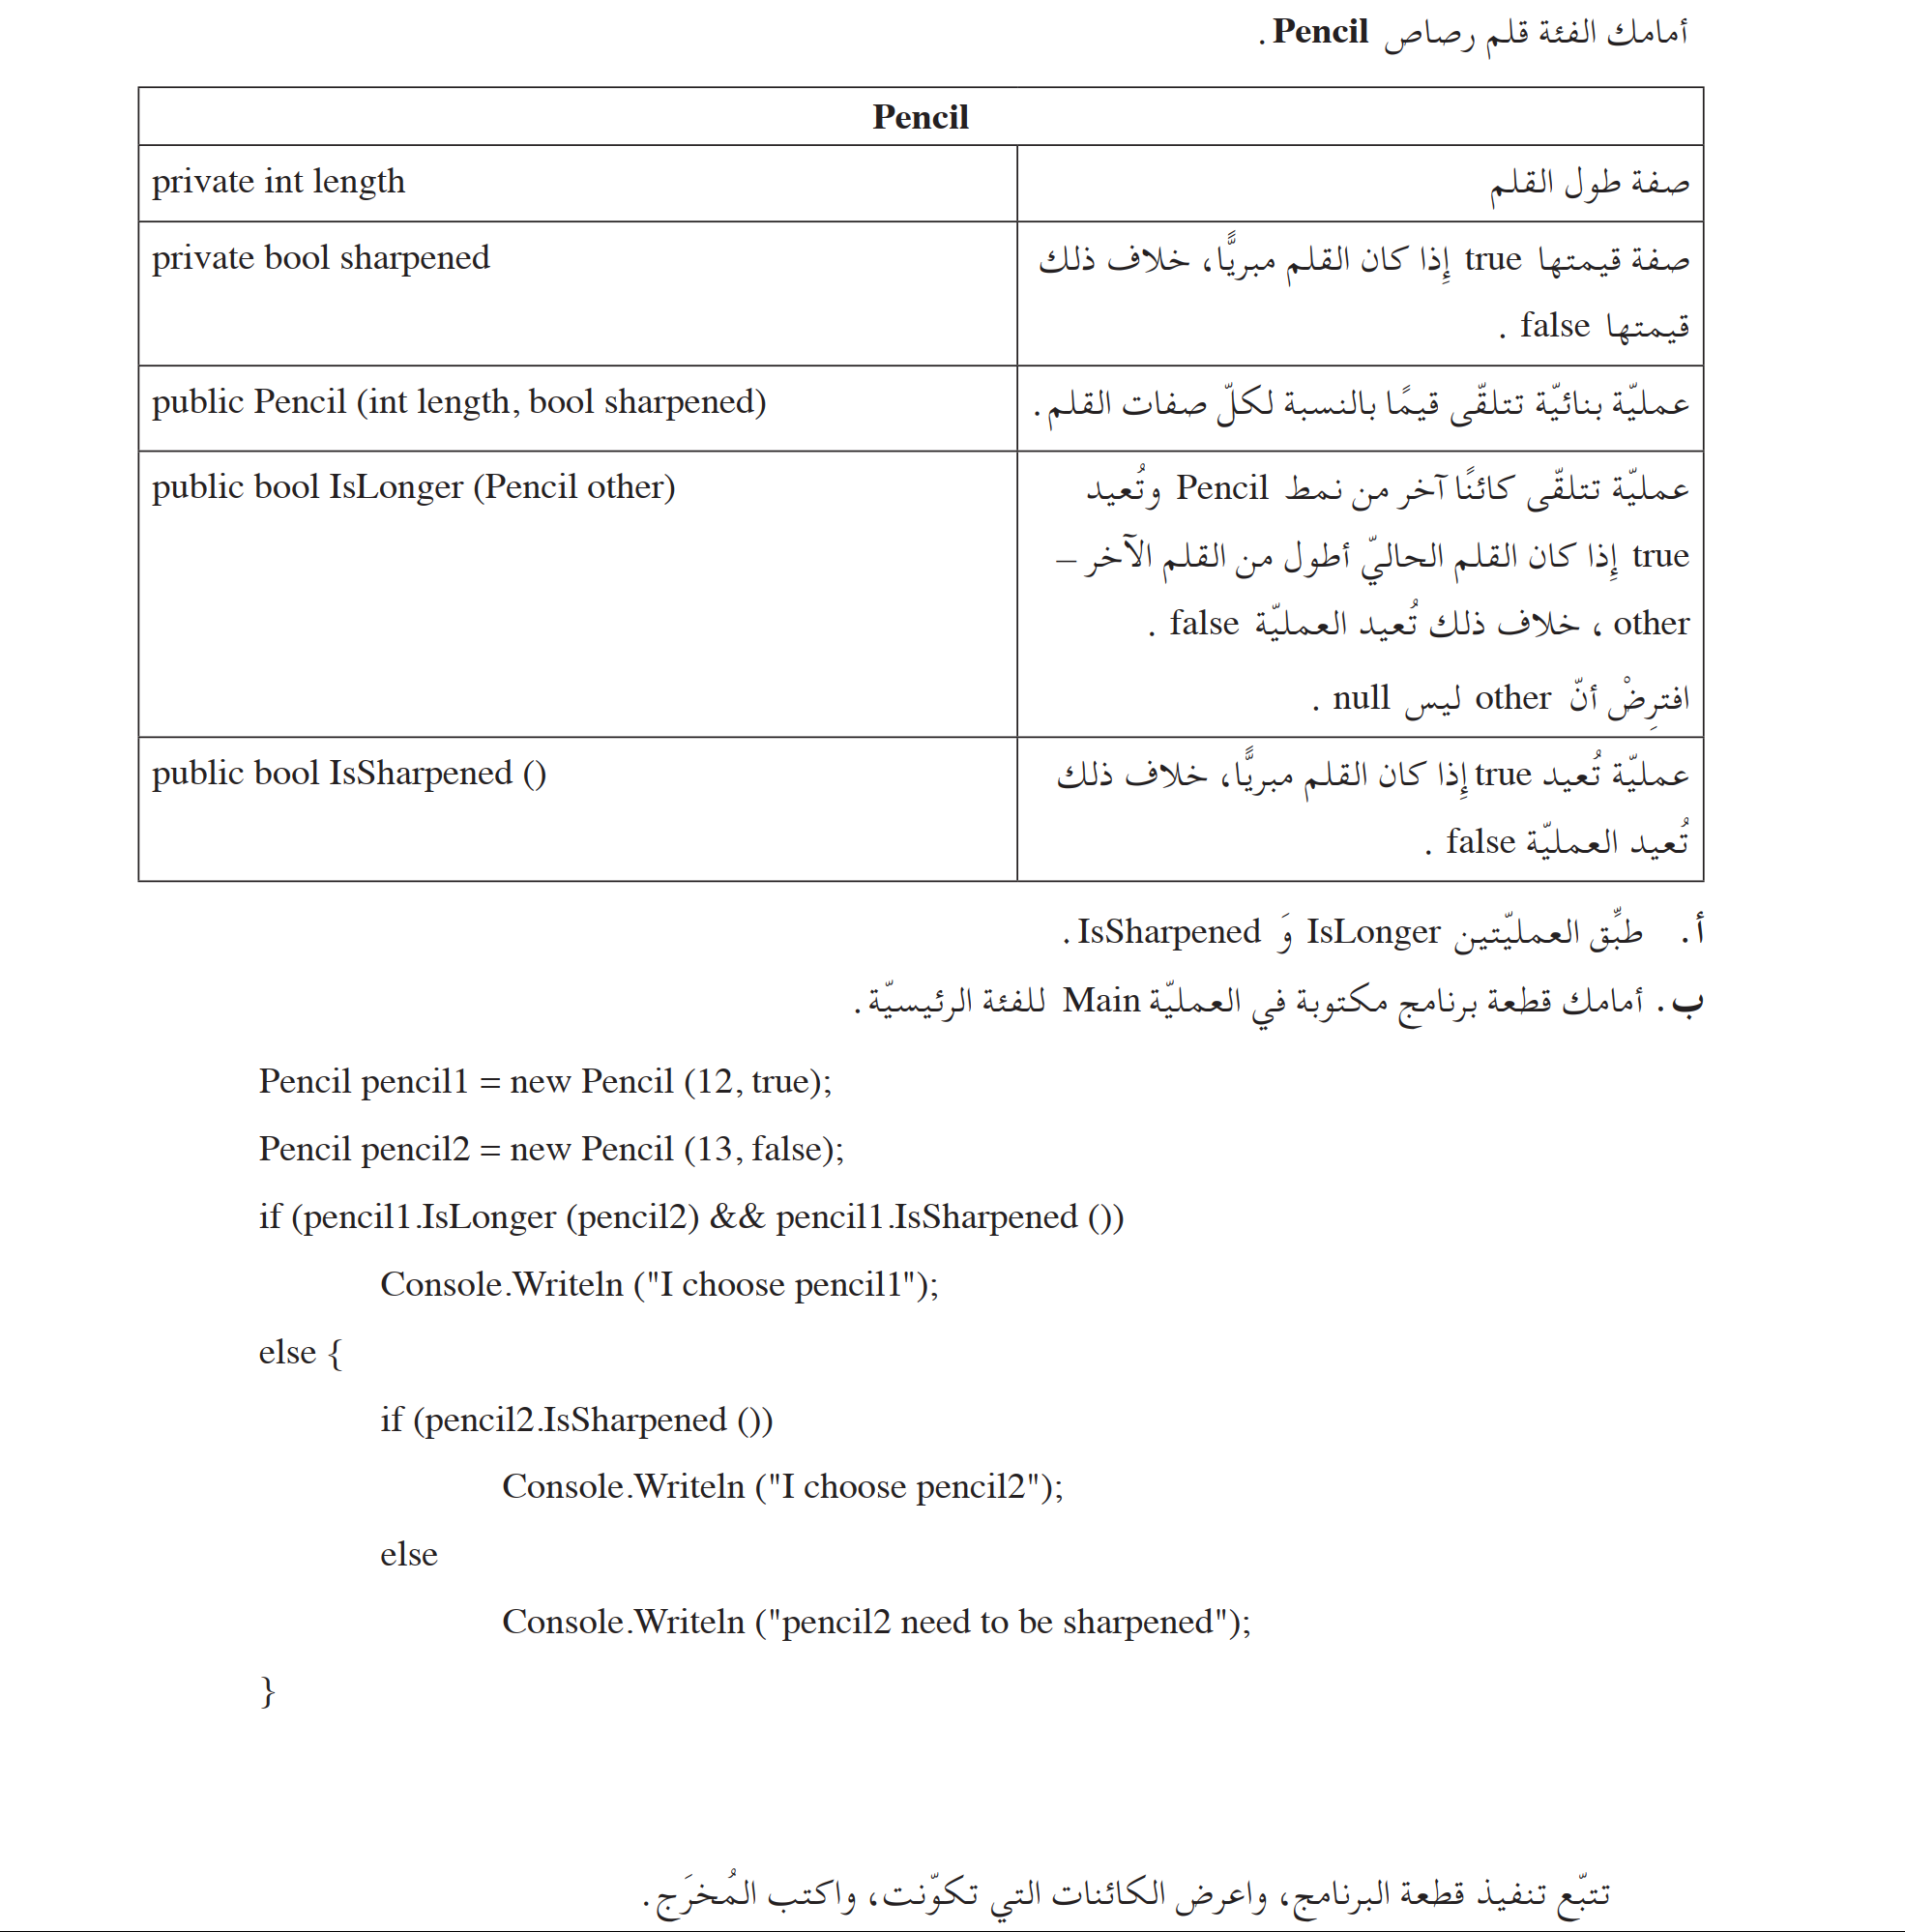
\includegraphics[width=0.9\paperwidth,keepaspectratio]{../../../bagrut_questions/basics/classes0_2020_899381b_1.png }%
% }%

% % \item \textbf{السؤال الثاني} \\
% % أمامك الفئة قلم رصاص \textenglish{Pencil}.

% % \begin{center}
% % \renewcommand{\arraystretch}{1.5}
% % \begin{tabular}{|p{9.5cm}|l|}
% % \hline
% % \multicolumn{2}{|c|}{\textbf{\textenglish{Pencil}}} \\
% % \hline
% % صفة طول القلم & \textenglish{private int length} \\
% % \hline
% % صفة قيمتها \textenglish{true} إذا كان القلم مبريًّا، خلاف ذلك قيمتها \textenglish{false}. & \textenglish{private bool sharpened} \\
% % \hline
% % عمليّة بنائية تتلقّى قيمًا بالنسبة لكلّ صفات القلم. & \textenglish{public Pencil(int length, bool sharpened)} \\
% % \hline
% % عمليّة تتلقّى كائنًا آخر من نمط \textenglish{Pencil} وتُعيد \textenglish{true} إذا كان القلم الحالي أطول من القلم الآخر - \textenglish{other}، خلاف ذلك تُعيد العمليّة \textenglish{false}. \newline افترض أنّ \textenglish{other} ليس \textenglish{null}. & \textenglish{public bool IsLonger(Pencil other)} \\
% % \hline
% % عمليّة تُعيد \textenglish{true} إذا كان القلم مبريًّا، خلاف ذلك تُعيد العمليّة \textenglish{false}. & \textenglish{public bool IsSharpened()} \\
% % \hline
% % \end{tabular}
% % \end{center}

% % \begin{enumerate}
% %     \item طبّق العمليّتين \textenglish{IsLonger} وَ \textenglish{IsSharpened}.
% %     \item أمامك قطعة برنامج مكتوبة في العمليّة \textenglish{Main} للفئة الرئيسيّة:
% % \end{enumerate}

% % \begin{boxCode}
% % \begin{english}
% % \begin{minted}{csharp}
% % Pencil pencil1 = new Pencil(12, true);
% % Pencil pencil2 = new Pencil(13, false);

% % if (pencil1.IsLonger(pencil2) && pencil1.IsSharpened())
% %     Console.WriteLine("I choose pencil1");
% % else
% % {
% %     if (pencil2.IsSharpened())
% %         Console.WriteLine("I choose pencil2");
% %     else
% %         Console.WriteLine("pencil2 need to be sharpened");
% % }
% % \end{minted}
% % \end{english}
% % \end{boxCode}

% % تتبّع تنفيذ قطعة البرنامج، واعرض الكائنات التي تكوّنت، واكتب المُخْرَج.

% % \vspace{1cm}

% % % ================= مساحة الكائنات وجدول المتابعة (يمكن نقله لصفحة الإجابات) =================
% % \textbf{\large الكائنات التي تكوّنت:}
% % \vspace{3cm} % مساحة فارغة لرسم الكائنات

% % \textbf{\large جدول المتابعة:}
% % \begin{center}
% %     \renewcommand{\arraystretch}{1.5}
% %     \begin{tabular}{|c|c|c|}
% %         \hline
% %         \textbf{\textenglish{pencil1.IsLonger(pencil2)}} & \textbf{\textenglish{pencil1.IsSharpened()}} & \textbf{\textenglish{pencil2.IsSharpened()}} \\
% %         \hline
% %         \hspace{3.5cm} & \hspace{3.5cm} & \hspace{3.5cm} \\ \hline
% %          & & \\ \hline
% %          & & \\ \hline
% %          & & \\ \hline
% %     \end{tabular}
% % \end{center}

% % \vspace{1cm}
% % \noindent \textbf{\large المُخْرَج (الطباعة):} \underline{\hspace{6cm}}

% %%%%%%%%%%%%%%%%%%%%%%%%%%%%%%%%%%%%%%%%%%%%%%%%%%%%%%%%%%%%%%%%%%%%%%%%%%%%%%%%%%%%%%%%%%%%%%%%%%%%%%%
% \clearpage
% \section*{الفصل الثاني}

% \textbf{السؤال الثالث} (30 علامة) \\
% يضمّ مجلس إقليميّ معيّن 10 بلدات، يُشار إليها بالأعداد الترتيبيّة من 0 حتّى 9. \\
% في المجلس الإقليميّ نوعان من التخفيضات في دفع الضرائب:
% \begin{itemize}
%     \item إذا كان عدد الأفراد في العائلة أكبر من 6، فإنّها تحصل على تخفيض بقيمة 100 شيكل.
%     \item إذا كان في العائلة طلّاب ثانويّون، فإنّها تحصل على تخفيض بقيمة 40 شيكل مقابل كلّ طالب ثانويّ.
% \end{itemize}
% العائلة التي تستحقّ الحصول على نوعي التخفيضات، تحصل فقط على نوع التخفيض الأعلى من بينهما.

% \begin{enumerate}
%     \item[\textbf{أ.}] اكتب عمليّة خارجيّة تتلقّى بالنسبة لعائلة معيّنة عدد الأفراد وعدد الطلاب الثانويّين في العائلة. \\
%     تُعيد العمليّة مبلغ التخفيض الذي تستحقّ هذه العائلة الحصول عليه. إذا كانت العائلة لا تستحقّ الحصول على تخفيض -- تُعيد العمليّة 0.

%     \item[\textbf{ب.}] اكتب عمليّة خارجيّة تتلقّى عدد العائلات في بلدة معيّنة في المجلس الإقليميّ. \\
%     بالنسبة لكلّ عائلة، تستقبل العمليّة عدد الأفراد وعدد الطلاب الثانويّين فيها. \\
%     تُعيد العمليّة مجموع كلّ التخفيضات التي مُنِحت في البلدة. \\
%     عليك استعمال العمليّة التي كتبتها في البند "أ".

%     \item[\textbf{ج.}] معطاة مصفوفة أحادية الأبعاد \textenglish{rdc} بكبَر 10، يحوي كلّ واحد من حدودها المبلغ الذي يخصّصه المجلس الإقليميّ للتخفيضات لبلدة واحدة. على سبيل المثال، الحدّ في المصفوفة الذي مؤشّره 5 يحوي المبلغ الذي خصّصه المجلس الإقليميّ للتخفيضات للبلدة التي عددها الترتيبيّ 5. \\
%     اكتب برنامجًا (عمليّة رئيسيّة \textenglish{Main}) يستقبل بالنسبة لكلّ بلدة، عدد العائلات التي فيها. \\
%     يطبع البرنامج الأعداد الترتيبيّة للبلدات التي فيها مجموع التخفيضات التي مُنِحت في البلدة أكبر من المبلغ الذي خصّصه المجلس الإقليميّ للتخفيضات للبلدة. \\
%     عليك استعمال العمليّة التي كتبتها في البند "ب".
% \end{enumerate}

% \textbf{\underline{ملاحظات:}}
% \begin{itemize}[itemsep=0em]
%     \item لا حاجة لفحص سلامة المدخلات.
%     \item لا حاجة لاستقبال المصفوفة.
%     \item لا حاجة لفحص سلامة المصفوفة.
% \end{itemize}

% %%%%%%%%%%%%%%%%%%%%%%%%%%%%%%%%%%%%%%%%%%%%%%%%%%%%%%%%%%%%%%%%%%%%%%%%%%%%%%%%%%%%%%%%%%%%%%%%%%%%%%%
% \clearpage
% \textbf{السؤال الرابع} (30 علامة) \\
% % \subsection*{سؤال 8 امتحان 899222 سنة 2017}
\addcontentsline{toc}{subsection}{سؤال 8 امتحان 899222 سنة 2017}

\noindent
\makebox[\textwidth][c]{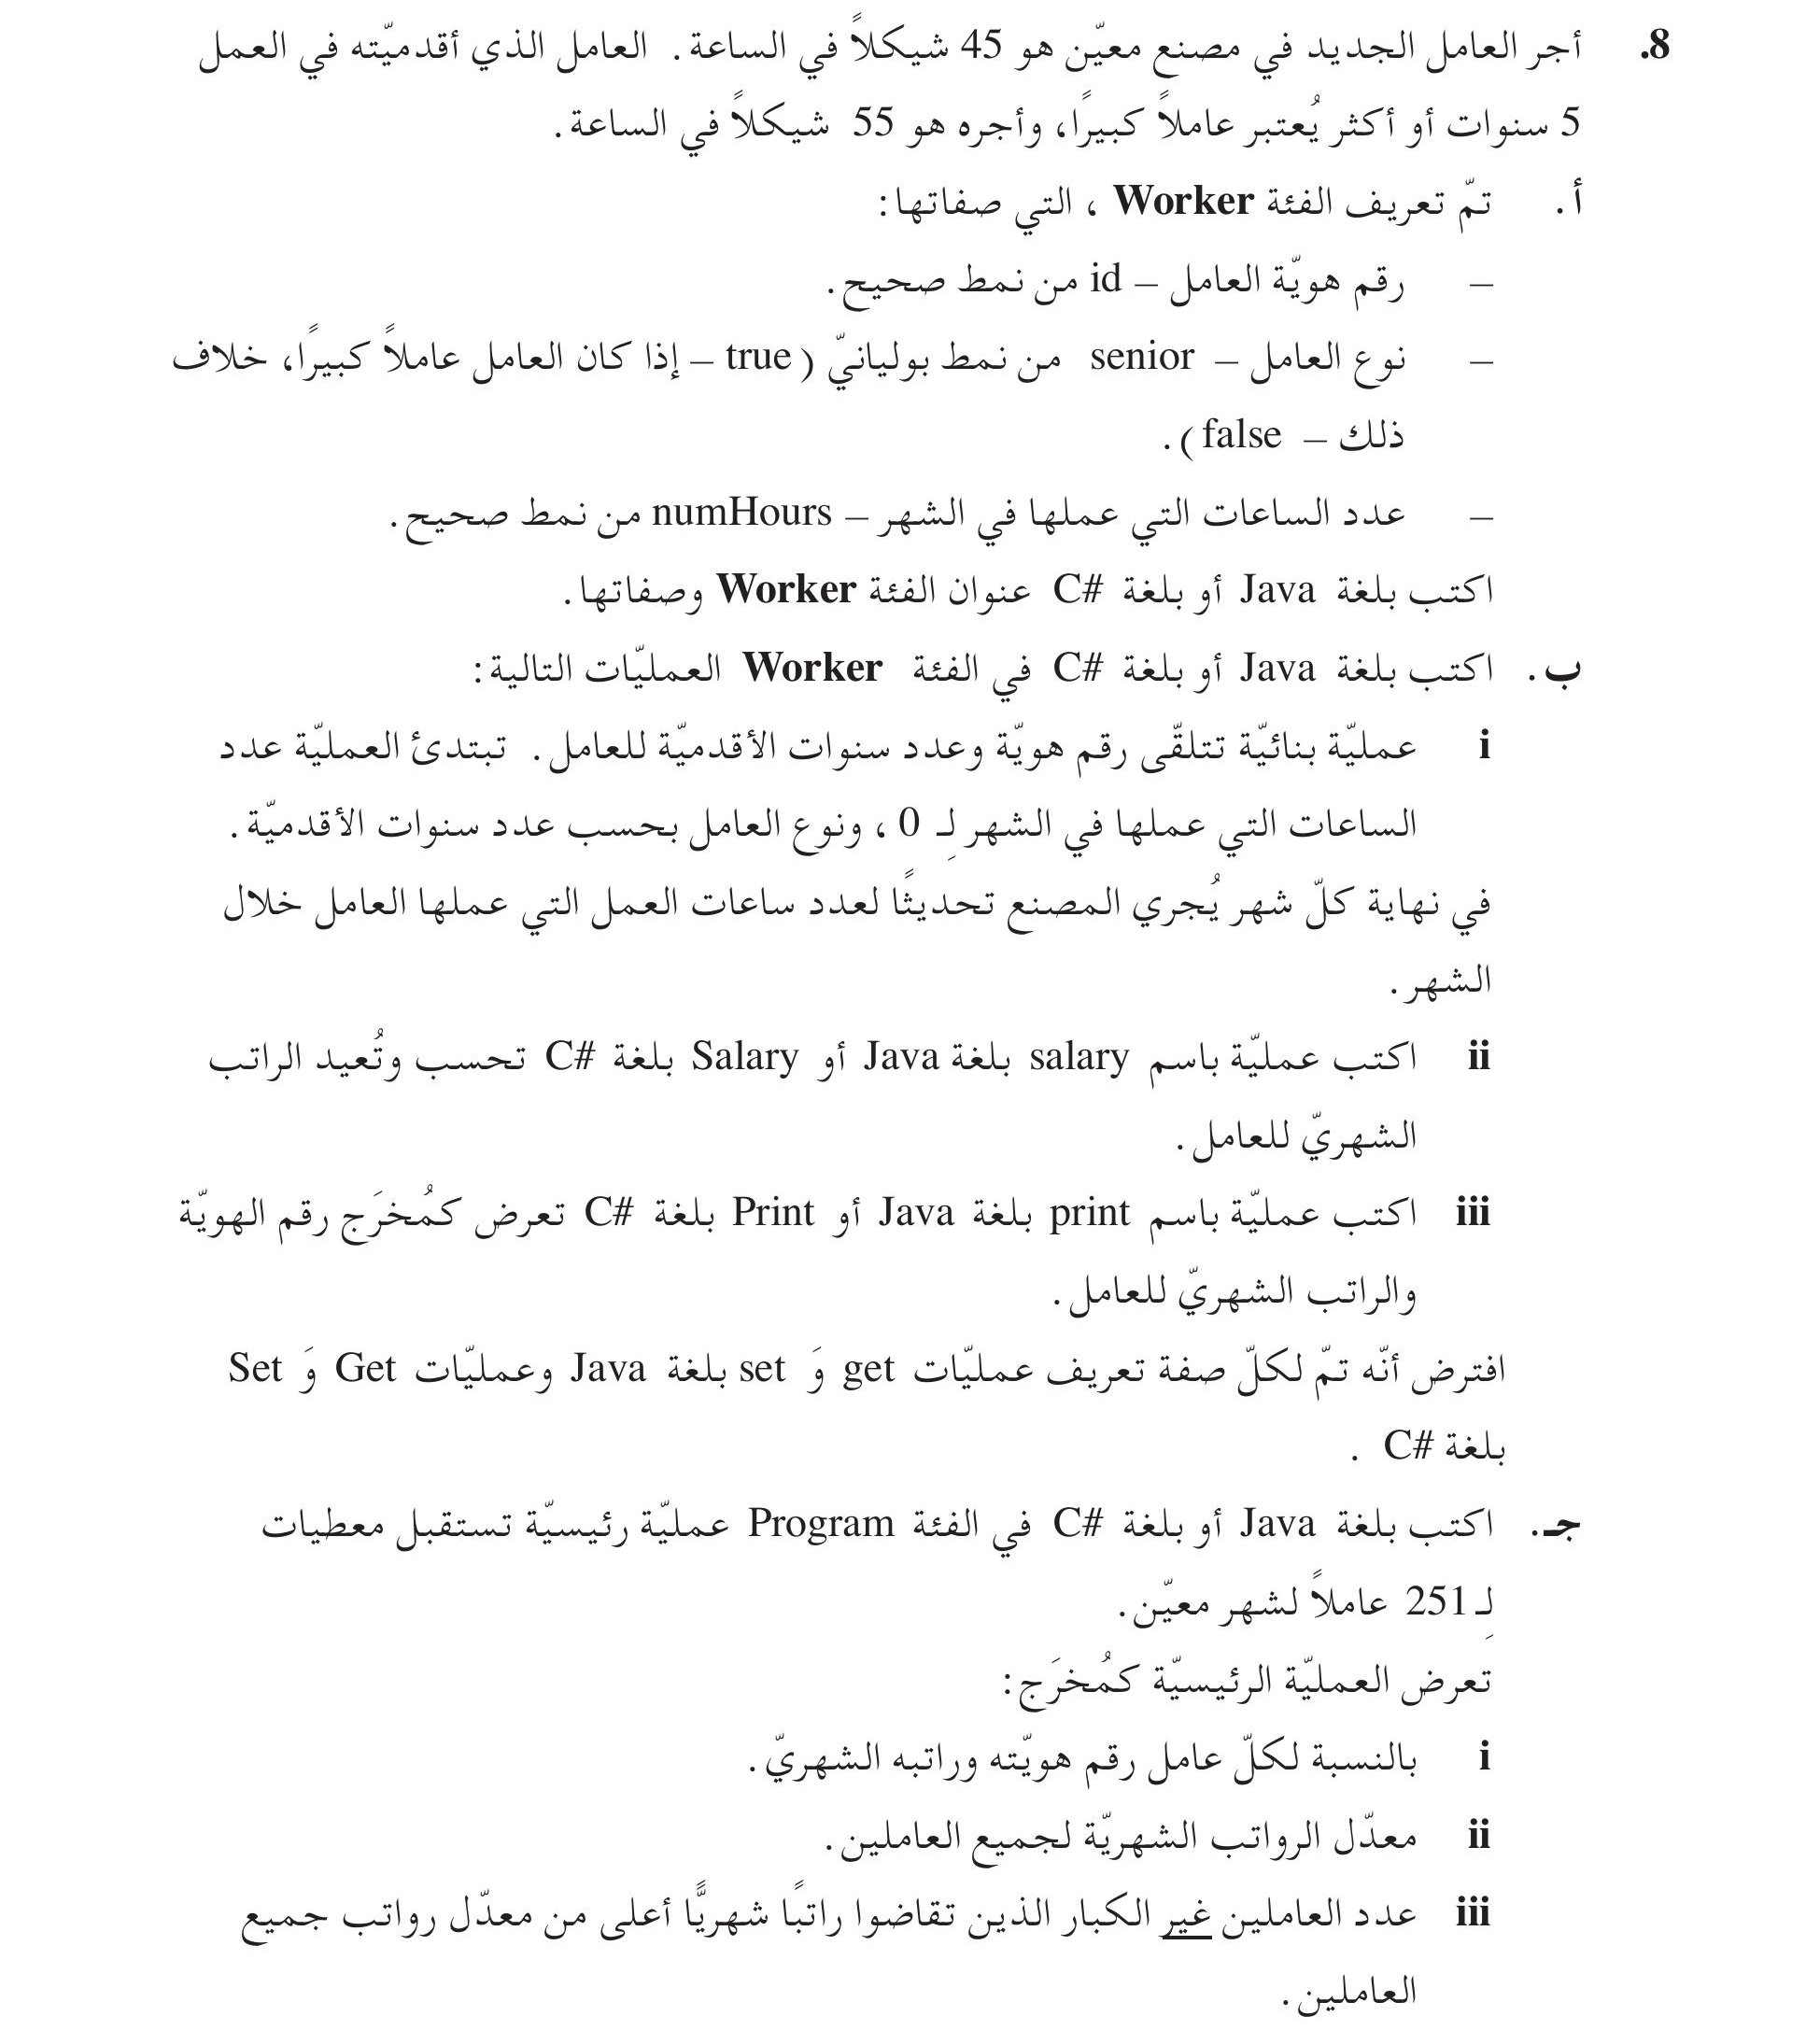
\includegraphics[width=0.9\paperwidth,keepaspectratio]{ ../../../bagrut_questions/basics/classes1_2017_899222_8.jpg }%
}%


\ifwithsols
{\small
\begin{boxSolution}[سؤال 8 امتحان 899222 سنة 2017]
\begin{boxCode}
\begin{english}
\begin{minted}{csharp}
class Worker
{
    private int id;
    private bool senior;
    private int numHours;

    public Worker(int id, int years)
    {
        this.id = id;
        if (years >= 5)
            this.senior = true;
        else
            this.senior = false;
        this.numHours = 0;
    }

    public int Salary()
    {
        if (this.senior)
            return this.numHours * 55;
        return this.numHours * 45;
    }

    public void Print()
    {
        Console.WriteLine(this.id + " " + this.Salary());
    }
    public void SetNumHours(int numHours) { this.numHours = numHours; }
    public bool GetSenior() { return this.senior; }
}
\end{minted}
\end{english}
\end{boxCode}
\end{boxSolution}

\begin{boxSolution}[سؤال 8 امتحان 899222 سنة 2017 - تكملة]
\begin{boxCode}
\begin{english}
\begin{minted}{csharp}
class Program
{
    public static void Main(string[] args)
    {
        Worker[] arr = new Worker[251];
        int sum = 0;

        for (int i = 0; i < 251; i++)
        {
            int id = int.Parse(Console.ReadLine());
            int years = int.Parse(Console.ReadLine());
            int hours = int.Parse(Console.ReadLine());

            arr[i] = new Worker(id, years);
            arr[i].SetNumHours(hours);

            arr[i].Print();
            sum += arr[i].Salary();
        }

        double avg = (double)sum / 251;
        Console.WriteLine(avg);

        int count = 0;
        for (int i = 0; i < 251; i++)
        {
            if (!arr[i].GetSenior() && arr[i].Salary() > avg)
            {
                count++;
            }
        }
        Console.WriteLine(count);
    }
}
\end{minted}
\end{english}
\end{boxCode}
\end{boxSolution}
}
\clearpage
\fi

% أجر العامل الجديد في مصنع معيّن هو 45 شيكلاً في الساعة. العامل الذي أقدميّته في العمل 5 سنوات أو أكثر يُعتبر عاملًا كبيرًا، وأجره هو 55 شيكلاً في الساعة.

% \begin{enumerate}
%     \item[\textbf{أ.}] تمّ تعريف الفئة \textenglish{Worker}، التي صفاتها:
%     \begin{itemize}
%         \item رقم هويّة العامل - \textenglish{id} من نمط صحيح.
%         \item نوع العامل - \textenglish{senior} من نمط بولياني (\textenglish{true} - إذا كان العامل عاملًا كبيرًا، خلاف ذلك - \textenglish{false}).
%         \item عدد الساعات التي عملها في الشهر - \textenglish{numHours} من نمط صحيح.
%     \end{itemize}
%     اكتب عنوان الفئة \textenglish{Worker} وصفاتها.

%     \item[\textbf{ب.}] اكتب في الفئة \textenglish{Worker} العمليّات التالية:
%     \begin{enumerate}
%         \item[\textbf{i.}] عمليّة بنائية تتلقّى رقم هويّة وعدد سنوات الأقدميّة للعامل. تبتدئ العمليّة عدد الساعات التي عملها في الشهر بـ 0، ونوع العامل بحسب عدد سنوات الأقدميّة. \\
%         في نهاية كلّ شهر يُجري المصنع تحديثًا لعدد ساعات العمل التي عملها العامل خلال الشهر.
%         \item[\textbf{ii.}] اكتب عمليّة باسم \textenglish{Salary} تحسب وتُعيد الراتب الشهريّ للعامل.
%         \item[\textbf{iii.}] اكتب عمليّة باسم \textenglish{Print} تعرض كمُخْرَج رقم الهويّة والراتب الشهريّ للعامل.
%     \end{enumerate}
%     افترض أنّه تمّ لكلّ صفة تعريف عمليّات \textenglish{Get} وَ \textenglish{Set} .

%     \item[\textbf{ج.}] اكتب في الفئة \textenglish{Program} عمليّة رئيسيّة تستقبل معطيات لـ 251 عاملًا لشهر معيّن. \\
%     تعرض العمليّة الرئيسيّة كمُخْرَج:
%     \begin{enumerate}
%         \item[\textbf{i.}] بالنسبة لكلّ عامل رقم هويّته وراتبه الشهريّ.
%         \item[\textbf{ii.}] معدّل الرواتب الشهريّة لجميع العاملين.
%         \item[\textbf{iii.}] عدد العاملين \underline{غير الكبار} الذين تقاضوا راتبًا شهريًّا أعلى من معدّل رواتب جميع العاملين.
%     \end{enumerate}
% \end{enumerate}


% %%%%%%%%%%%%%%%%%%%%%%%%%%%%%%%%%%%%%%%%%%%%%%%%%%%%%%%%%%%%%%%%%%%%%%%%%%%%%%%%%%%%%%%%%%%%%%%%%%%%%%%%%%%
% \clearpage
% \textbf{السؤال الخامس} (30 علامة)
% % \subsection*{سؤال 9 امتحان 899222 سنة 2017}
\addcontentsline{toc}{subsection}{سؤال 9 امتحان 899222 سنة 2017}

\noindent
\makebox[\textwidth][c]{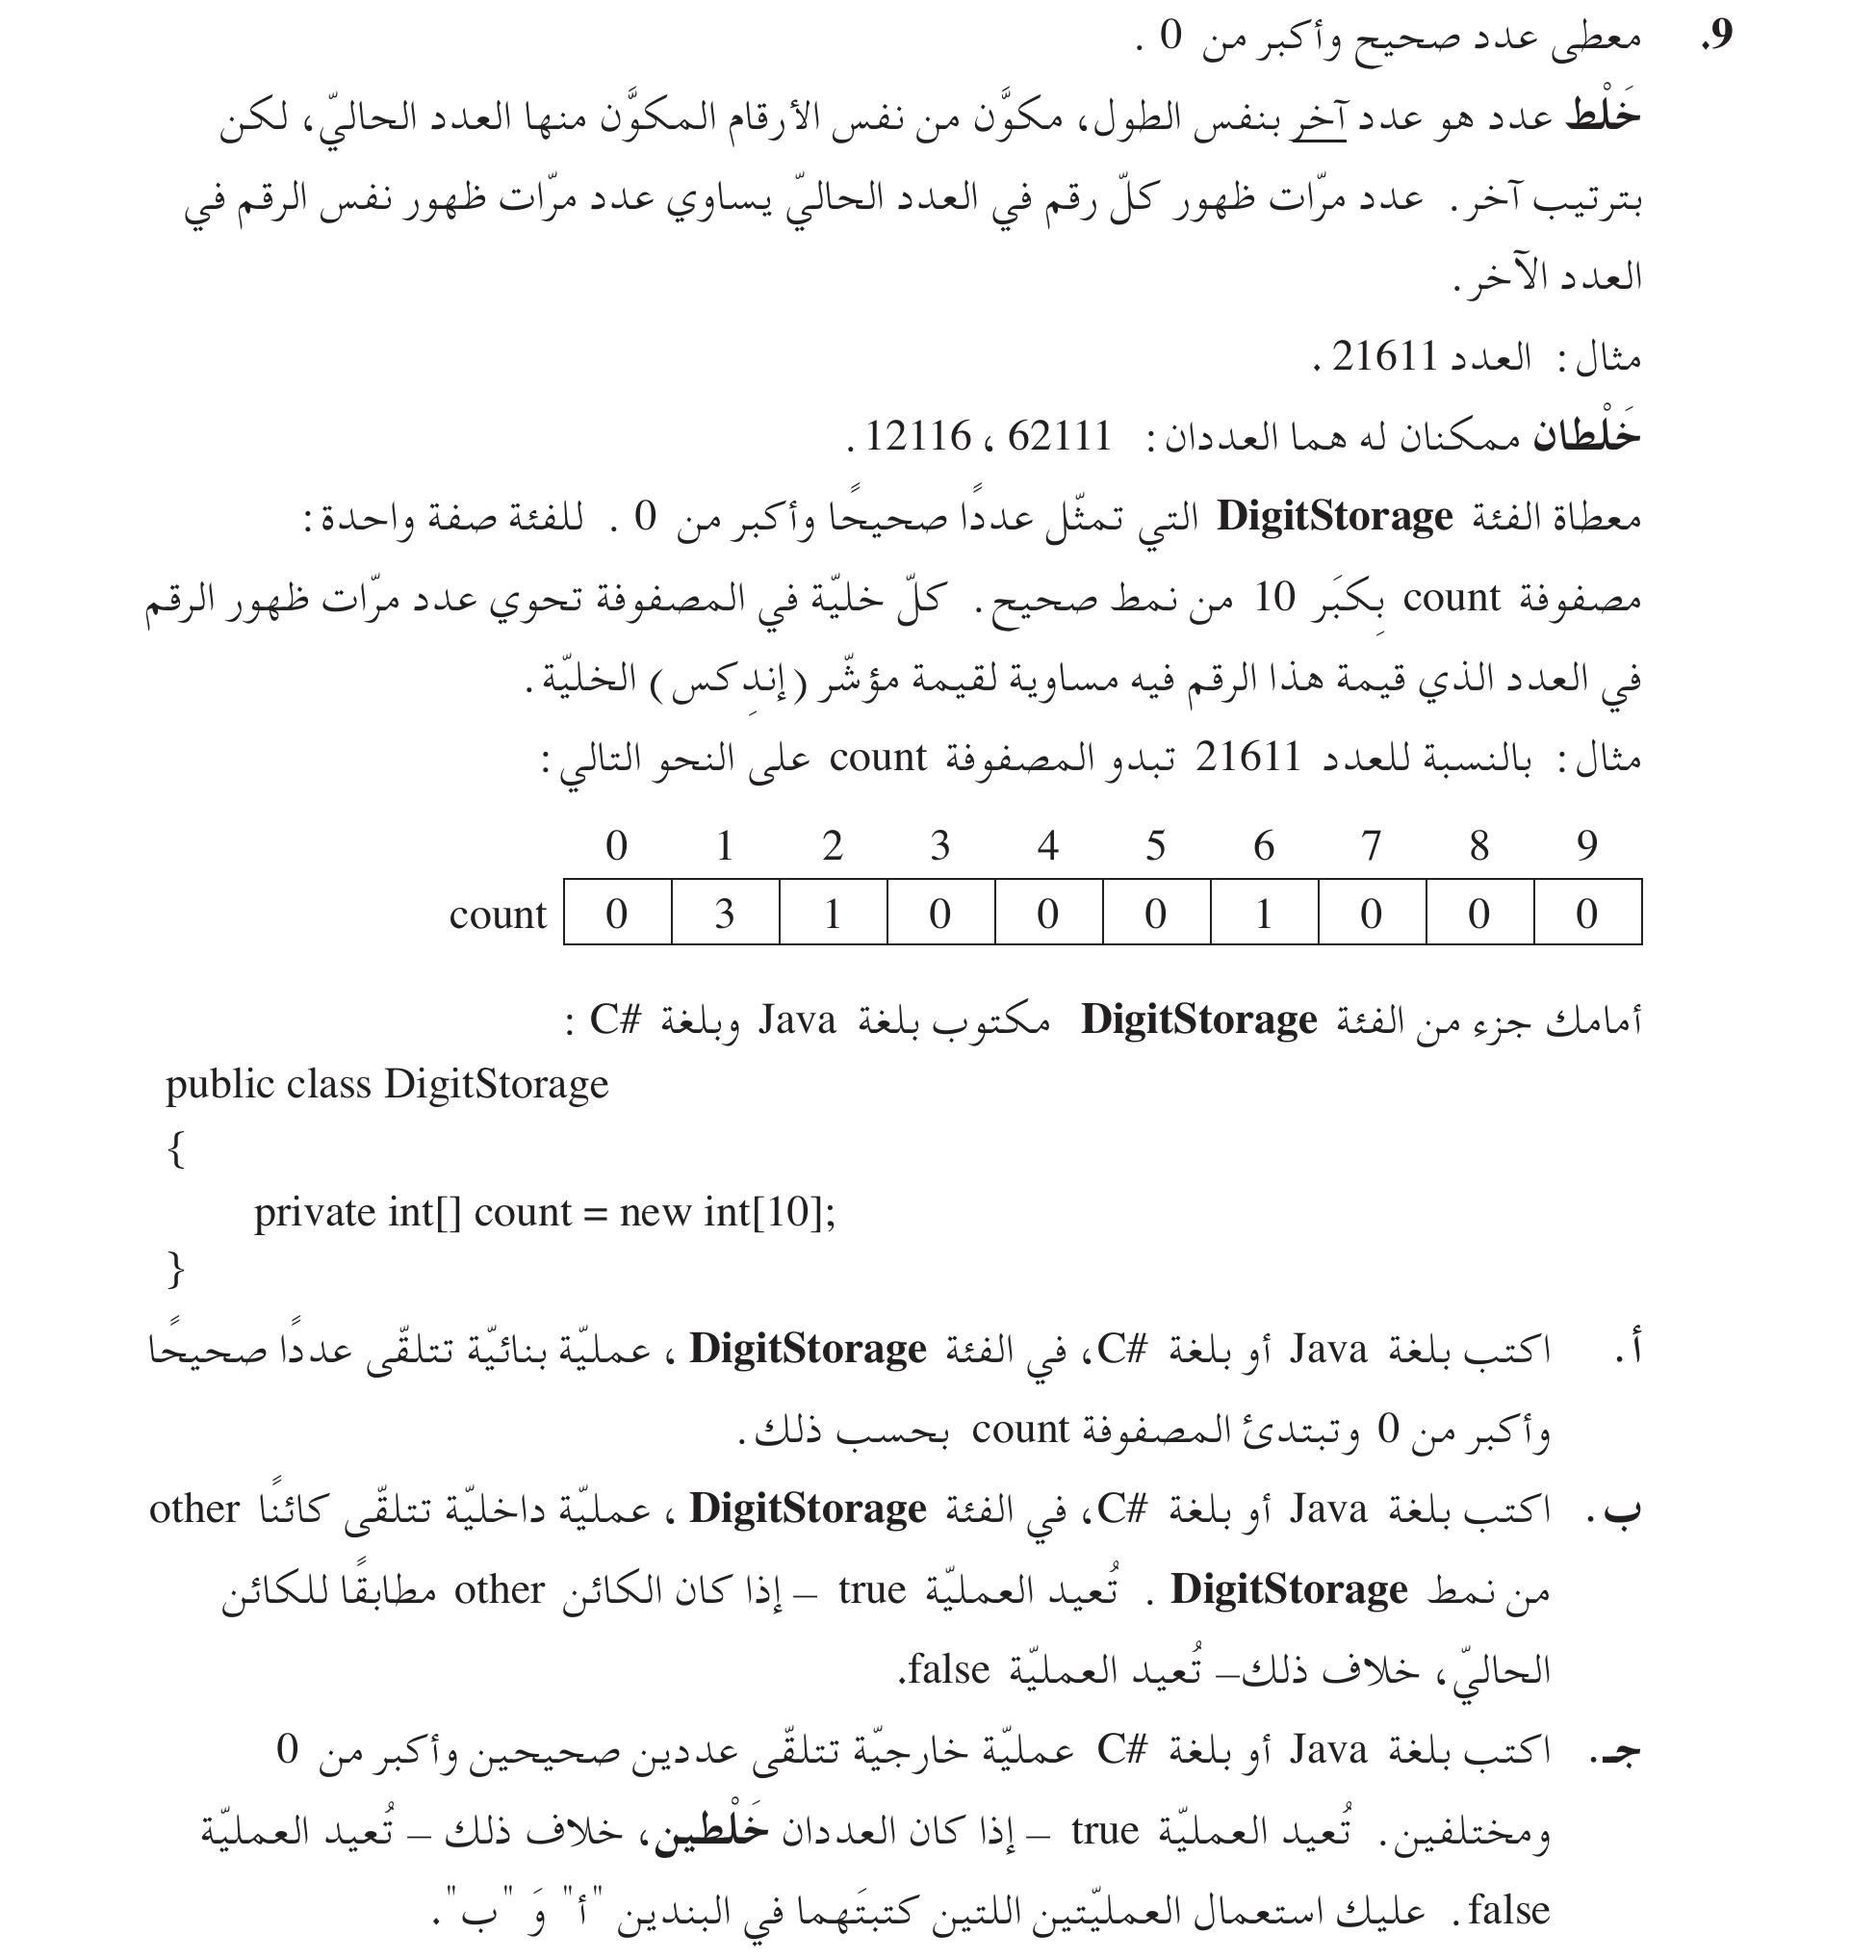
\includegraphics[width=0.9\paperwidth,keepaspectratio]{ ../../../bagrut_questions/basics/classes2_2017_899222_9.jpg }%
}%


\ifwithsols
{\small
\begin{boxSolution}[سؤال 9 امتحان 899222 سنة 2017]
\begin{boxCode}
\begin{english}
\begin{minted}{csharp}
public class DigitStorage
{
    private int[] count = new int[10];

    public DigitStorage(int num)
    {
        while (num > 0)
        {
            this.count[num % 10]++;
            num = num / 10;
        }
    }

    public bool IsIdentical(DigitStorage other)
    {
        for (int i = 0; i < 10; i++)
        {
            if (this.count[i] != other.count[i])
                return false;
        }
        return true;
    }
}

class Program
{
    public static bool IsMix(int num1, int num2)
    {
        DigitStorage d1 = new DigitStorage(num1);
        DigitStorage d2 = new DigitStorage(num2);

        return d1.IsIdentical(d2);
    }
}
\end{minted}
\end{english}
\end{boxCode}
\end{boxSolution}
}
\clearpage
\fi


% معطى عدد صحيح وأكبر من 0. \\
% \textbf{خَلْط} عدد هو عدد \underline{آخر} بنفس الطول، مكوّن من نفس الأرقام المكوّن منها العدد الحاليّ، لكن بترتيب آخر. عدد مرّات ظهور كلّ رقم في العدد الحاليّ يساوي عدد مرّات ظهور نفس الرقم في العدد الآخر. \\
% مثال: العدد 21611. \\
% \textbf{خَلْطان} ممكنان له هما العددان: 62111 ، 12116.

% معطاة الفئة \textenglish{DigitStorage} التي تمثّل عددًا صحيحًا وأكبر من 0. للفئة صفة واحدة: \\
% مصفوفة \textenglish{count} بكِبَر 10 من نمط صحيح. كلّ خليّة في المصفوفة تحوي عدد مرّات ظهور الرقم في العدد الذي قيمة هذا الرقم فيه مساوية لقيمة مؤشّر (إندكس) الخليّة. \\
% مثال: بالنسبة للعدد 21611 تبدو المصفوفة \textenglish{count} على النحو التالي:

% {\small
% \begin{english}
% \begin{center}
% \renewcommand{\arraystretch}{1.5}
% \setlength{\tabcolsep}{10pt}
% \begin{tabular}{c | c | c | c | c | c | c | c | c | c | c |}
% \multicolumn{1}{c}{} & \multicolumn{1}{c}{0} & \multicolumn{1}{c}{1} & \multicolumn{1}{c}{2} & \multicolumn{1}{c}{3} & \multicolumn{1}{c}{4} & \multicolumn{1}{c}{5} & \multicolumn{1}{c}{6} & \multicolumn{1}{c}{7} & \multicolumn{1}{c}{8} & \multicolumn{1}{c}{9} \\
% \cline{2-11}
% \textenglish{count} & 0 & 3 & 1 & 0 & 0 & 0 & 1 & 0 & 0 & 0 \\
% \cline{2-11}
% \end{tabular}
% \end{center}
% \end{english}
% }
% أمامك جزء من الفئة \textenglish{DigitStorage}:

% \begin{english}
% \begin{minted}{csharp}
% public class DigitStorage
% {
%     private int[] count = new int[10];
% }
% \end{minted}
% \end{english}

% \begin{enumerate}
%     \item[\textbf{أ.}] اكتب في الفئة \textenglish{DigitStorage}، عمليّة بنائيّة تتلقّى عددًا صحيحًا وأكبر من 0 وتبتدئ المصفوفة \textenglish{count} بحسب ذلك.

%     \item[\textbf{ب.}] اكتب في الفئة \textenglish{DigitStorage}، عمليّة داخليّة تتلقّى كائنًا \textenglish{other} من نمط \\ \textenglish{DigitStorage}. تُعيد العمليّة \textenglish{true} - إذا كان الكائن \textenglish{other} مطابقًا للكائن الحاليّ، خلاف ذلك - تُعيد العمليّة \textenglish{false}.

%     \item[\textbf{ج.}] اكتب عمليّة خارجيّة تتلقّى عددين صحيحين وأكبر من 0 ومختلفين. تُعيد العمليّة \textenglish{true} - إذا كان العددان \textbf{خَلْطَين}، خلاف ذلك - تُعيد العمليّة \textenglish{false}. عليك استعمال العمليّتين اللتين كتبتهما في البندين "أ" وَ "ب".
% \end{enumerate}

% \end{document}
